\documentclass[compress]{beamer}
\usepackage{ifthen,verbatim}

\newcommand{\isnote}{}
\xdefinecolor{lightyellow}{rgb}{1.,1.,0.25}
\xdefinecolor{darkblue}{rgb}{0.1,0.1,0.7}
\xdefinecolor{darkgreen}{rgb}{0.,0.5,0.}

%% Uncomment this to get annotations
%% \def\notes{\addtocounter{page}{-1}
%%            \renewcommand{\isnote}{*}
%% 	   \beamertemplateshadingbackground{lightyellow}{white}
%%            \begin{frame}
%%            \frametitle{Notes for the previous page (page \insertpagenumber)}
%%            \itemize}
%% \def\endnotes{\enditemize
%% 	      \end{frame}
%%               \beamertemplateshadingbackground{white}{white}
%%               \renewcommand{\isnote}{}}

%% Uncomment this to not get annotations
\def\notes{\comment}
\def\endnotes{\endcomment}

\setbeamertemplate{navigation symbols}{}
\setbeamertemplate{headline}{\mbox{ } \hfill
\begin{minipage}{5.5 cm}
\vspace{-0.75 cm} \small
\end{minipage} \hfill
\begin{minipage}{4.5 cm}
\vspace{-0.75 cm} \small
\begin{flushright}
\ifthenelse{\equal{\insertpagenumber}{1}}{}{Jim Pivarski \hspace{0.2 cm} \insertpagenumber\isnote/\pageref{numpages}}
\end{flushright}
\end{minipage}\mbox{\hspace{0.2 cm}}\includegraphics[height=1 cm]{../cmslogo} \hspace{0.1 cm} \includegraphics[height=1 cm]{../tamulogo} \hspace{0.01 cm} \vspace{-1.05 cm}}

\begin{document}
\begin{frame}
\vfill
\begin{center}
\textcolor{darkblue}{\Large Status of HIP Track-Based Alignment in the Endcap}

\vfill
\begin{columns}
\column{0.3\linewidth}
\begin{center}
\large
\textcolor{darkblue}{Jim Pivarski}

\vspace{0.2 cm}
Alexei Safonov
\end{center}
\end{columns}

\begin{columns}
\column{0.3\linewidth}
\begin{center}
\scriptsize
{\it Texas A\&M University}
\end{center}
\end{columns}

\vfill
26 June, 2009

\end{center}
\end{frame}

%% \begin{notes}
%% \item This is the annotated version of my talk.
%% \item If you want the version that I am presenting, download the one
%% labeled ``slides'' on Indico (or just ignore these yellow pages).
%% \item The annotated version is provided for extra detail and a written
%% record of comments that I intend to make orally.
%% \item Yellow notes refer to the content on the {\it previous} page.
%% \item All other slides are identical for the two versions.
%% \end{notes}

\small

\section*{Introduction}

\begin{frame}
\frametitle{Two unrelated topics}
\begin{itemize}\setlength{\itemsep}{0.75 cm}
\item Status of cosmics-during-collisions trigger
\item Updates in endcap disk alignment
\end{itemize}
%% \hspace{-0.83 cm} \textcolor{darkblue}{\Large Outline2}
\end{frame}

\section*{Trigger}

\begin{frame}
\frametitle{Cosmics-during-collisions}
\framesubtitle{Motivation}

\begin{itemize}\setlength{\itemsep}{0.25 cm}
\item Cosmic rays resolve ambiguities in collisions muons by the fact
  that they don't all point to the same spot
\begin{itemize}
\item ``small-scale'' track-source biases (within a small region of
  $\Delta \phi$,~$\Delta \theta$) are averaged over by cosmic rays,
  leaving only \\ ``global distortions'' (broad pattern across the
  whole detector)
\end{itemize}
\item Cosmic rays provide an ample source of high-momentum tracks
\begin{itemize}\setlength{\itemsep}{0.1 cm}
\item cosmic spectrum is $\mbox{(energy)}^{-2.7}$, rather than exponential
\item allows for $p_T > 100$~GeV alignments, $p_T > 500$~GeV
  diagnostics
\item Cosmic track-splitting is the only known way to quantify
  track resolution in all 5 track parameters
\end{itemize}
\item Despite the cosmic rays' ``verticalness'' disadvantage\ldots
\end{itemize}

\vfill Both tracker and muon alignment would be poorer if we stopped
collecting cosmic rays when the LHC turns on
\end{frame}

\begin{frame}
\frametitle{Cosmics-during-collisions}
\framesubtitle{Trigger issues}

\begin{itemize}\setlength{\itemsep}{0.35 cm}
\item Strange as it is to say it, cosmic ray signal is dwarfed by the
  $pp \to \mu X$ background rate
\item CMS triggers are not optimized for cosmic ray timing, either:
  $t(\mbox{bottom leg}) - t(\mbox{top leg}) \approx 3$~bunch crossings
\item Same problem with hit read-out: even given a trigger decision,
  it is not clear to me whether top and bottom hits would be put into
  the same event
\begin{itemize}
\item I need to ask the DT DAQ experts
\end{itemize}
\item Trigger time is discrete: we can only accept cosmic ray events
  that overlap bunch crossings, and therefore have pile-up
\end{itemize}
\end{frame}

\begin{frame}
\frametitle{Cosmics-during-collisions}
\framesubtitle{Trigger status}

\begin{itemize}
\item RPC L1 technical trigger has all of the elements needed to
  select 4-station coincidences on both sides of the barrel (roughly
  tracker-pointing), with the appropriate timing
\item Such a requirement should strongly discriminate against beam
  collision products: at most 10's of Hz, more likely 3--7~Hz
\item Quality cuts on standAloneMuon can be applied at HLT, though
  most of the rate reduction should happen at L1
\item Currently:
\begin{itemize}
\item high-level logic would need to be programmed in firmware
\item L1 emulator implemented in 3\_1\_0\_preX, but without the above
\item HLT path does not do any selection
\item efficiency (for cosmics) and fake-rate (for InclusiveMu) studies
  have begun (which will guide development of HLT cuts)
\end{itemize}
\item People responsible:
\begin{itemize}
\item L1 logic: RPC group (Flavio Loddo has offered)
\item Emulator: Andr\'es Osorio Oliveros (Universidad de Los Andes)
\item HLT and testing: Yohann Tschudi (Universit\'e Claude Bernard)
\end{itemize}
\end{itemize}
\end{frame}

\section*{Endcap alignment}
\begin{frame}
\begin{center}
\Huge \textcolor{blue}{Endcap alignment}
\end{center}
\end{frame}

\begin{frame}
\frametitle{Collected data}

\begin{minipage}{1.2\linewidth}
\begin{itemize}
\item Jump to the summary first: comparison of results from different sources
\item Any column might have an overall minus sign (differences in definitions)
\end{itemize}
\end{minipage}

\vfill
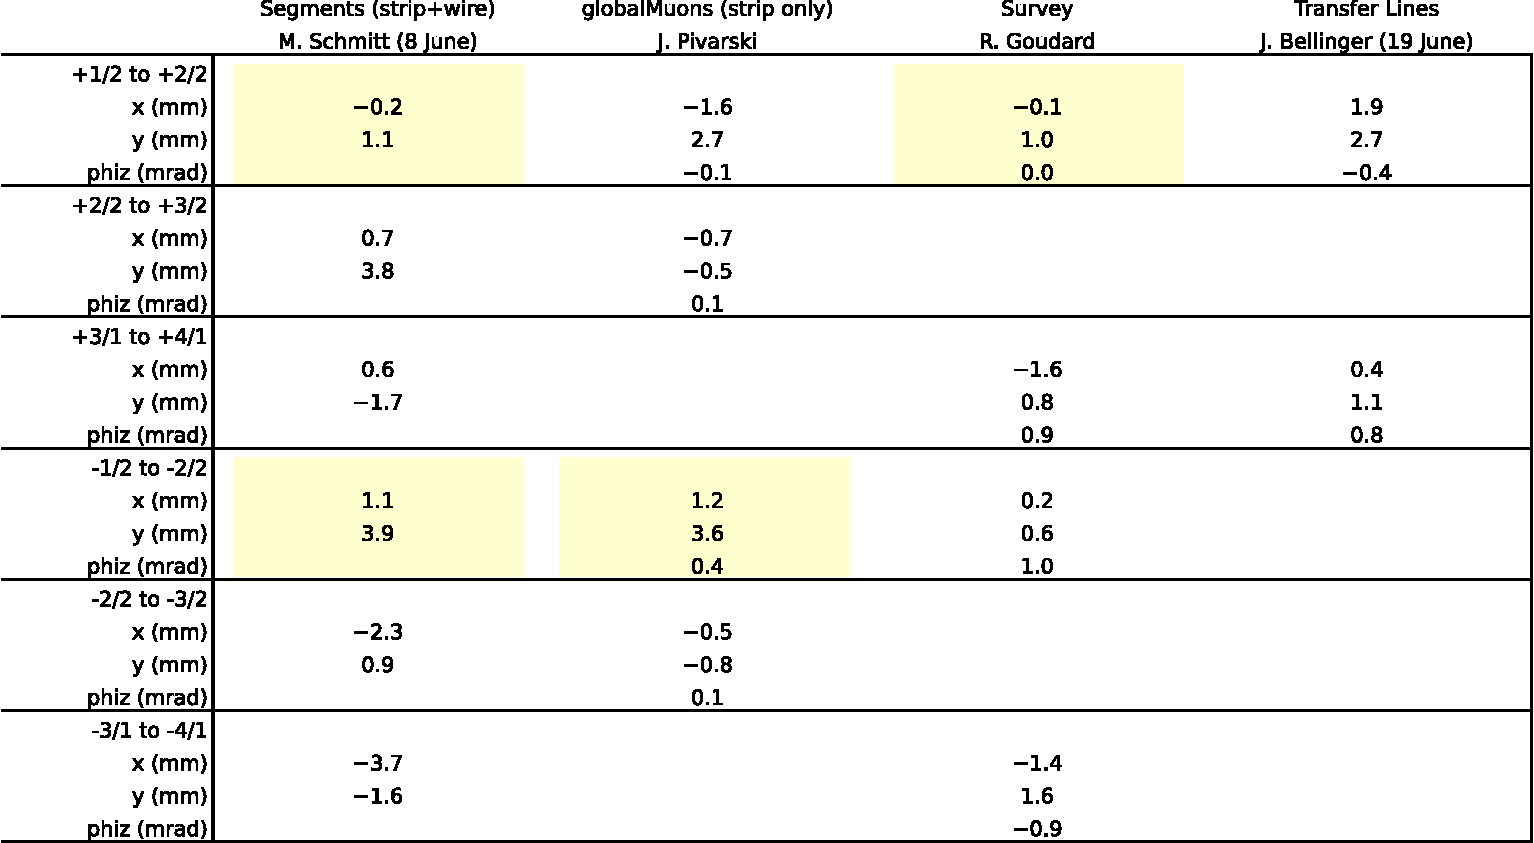
\includegraphics[width=\linewidth]{table.pdf}
\end{frame}

\begin{frame}
\frametitle{Where the data came from}

\begin{itemize}\setlength{\itemsep}{0.25 cm}
\item Segments (strip$+$wire): means of the histograms \\ (ignores sine trend from $\phi_z$)

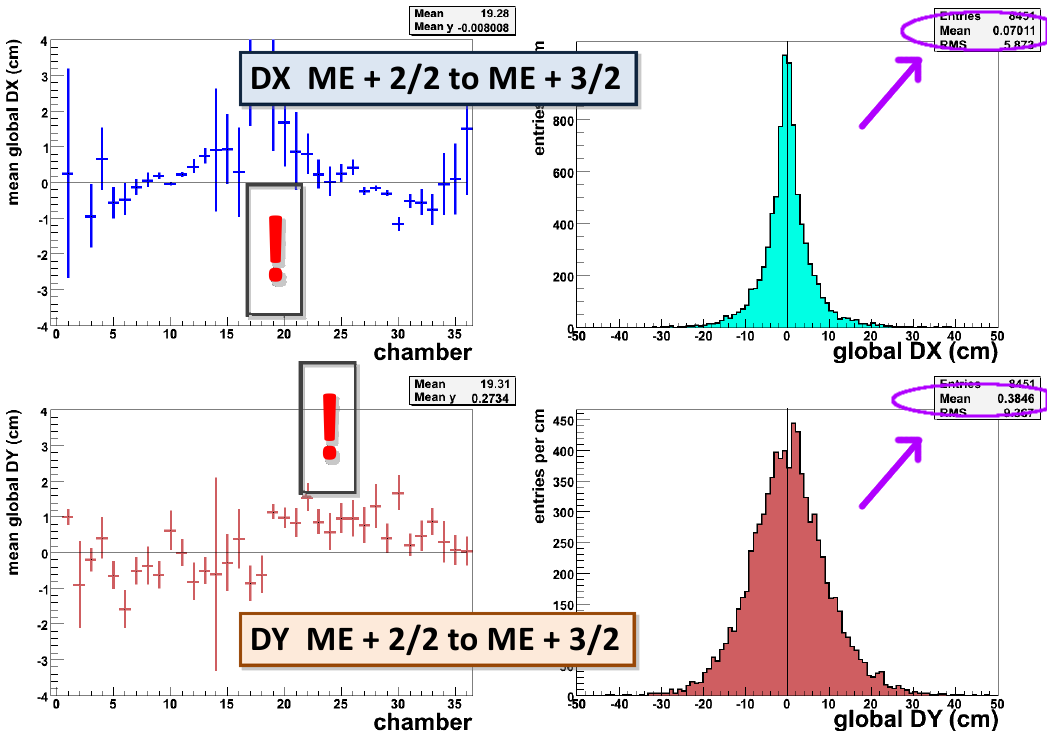
\includegraphics[width=0.65\linewidth]{global_residuals.png}

\item globalMuons (strip only): station 2 $\to$ 3 are residuals {\it differences}

\item Survey: soon-to-be-published note, Rapha\"el says they are preliminary, but $x$, $y$, $\phi_z$ are fairly well established

\item Transfer lines: table in presentation
\end{itemize}
\end{frame}

\begin{frame}
\frametitle{Map plots for CSCs}

\begin{itemize}
\item These are like the maps of the barrel (showing all ME$n$/2)
\begin{itemize}
\item raw hit distribution is the blue scale
\item black points are the means
\item dashed lines are the chamber boundaries
\end{itemize}
\item Note agreement between 2/2 and 3/2 in $x$ (not $\phi_y$)
\end{itemize}


\only<1>{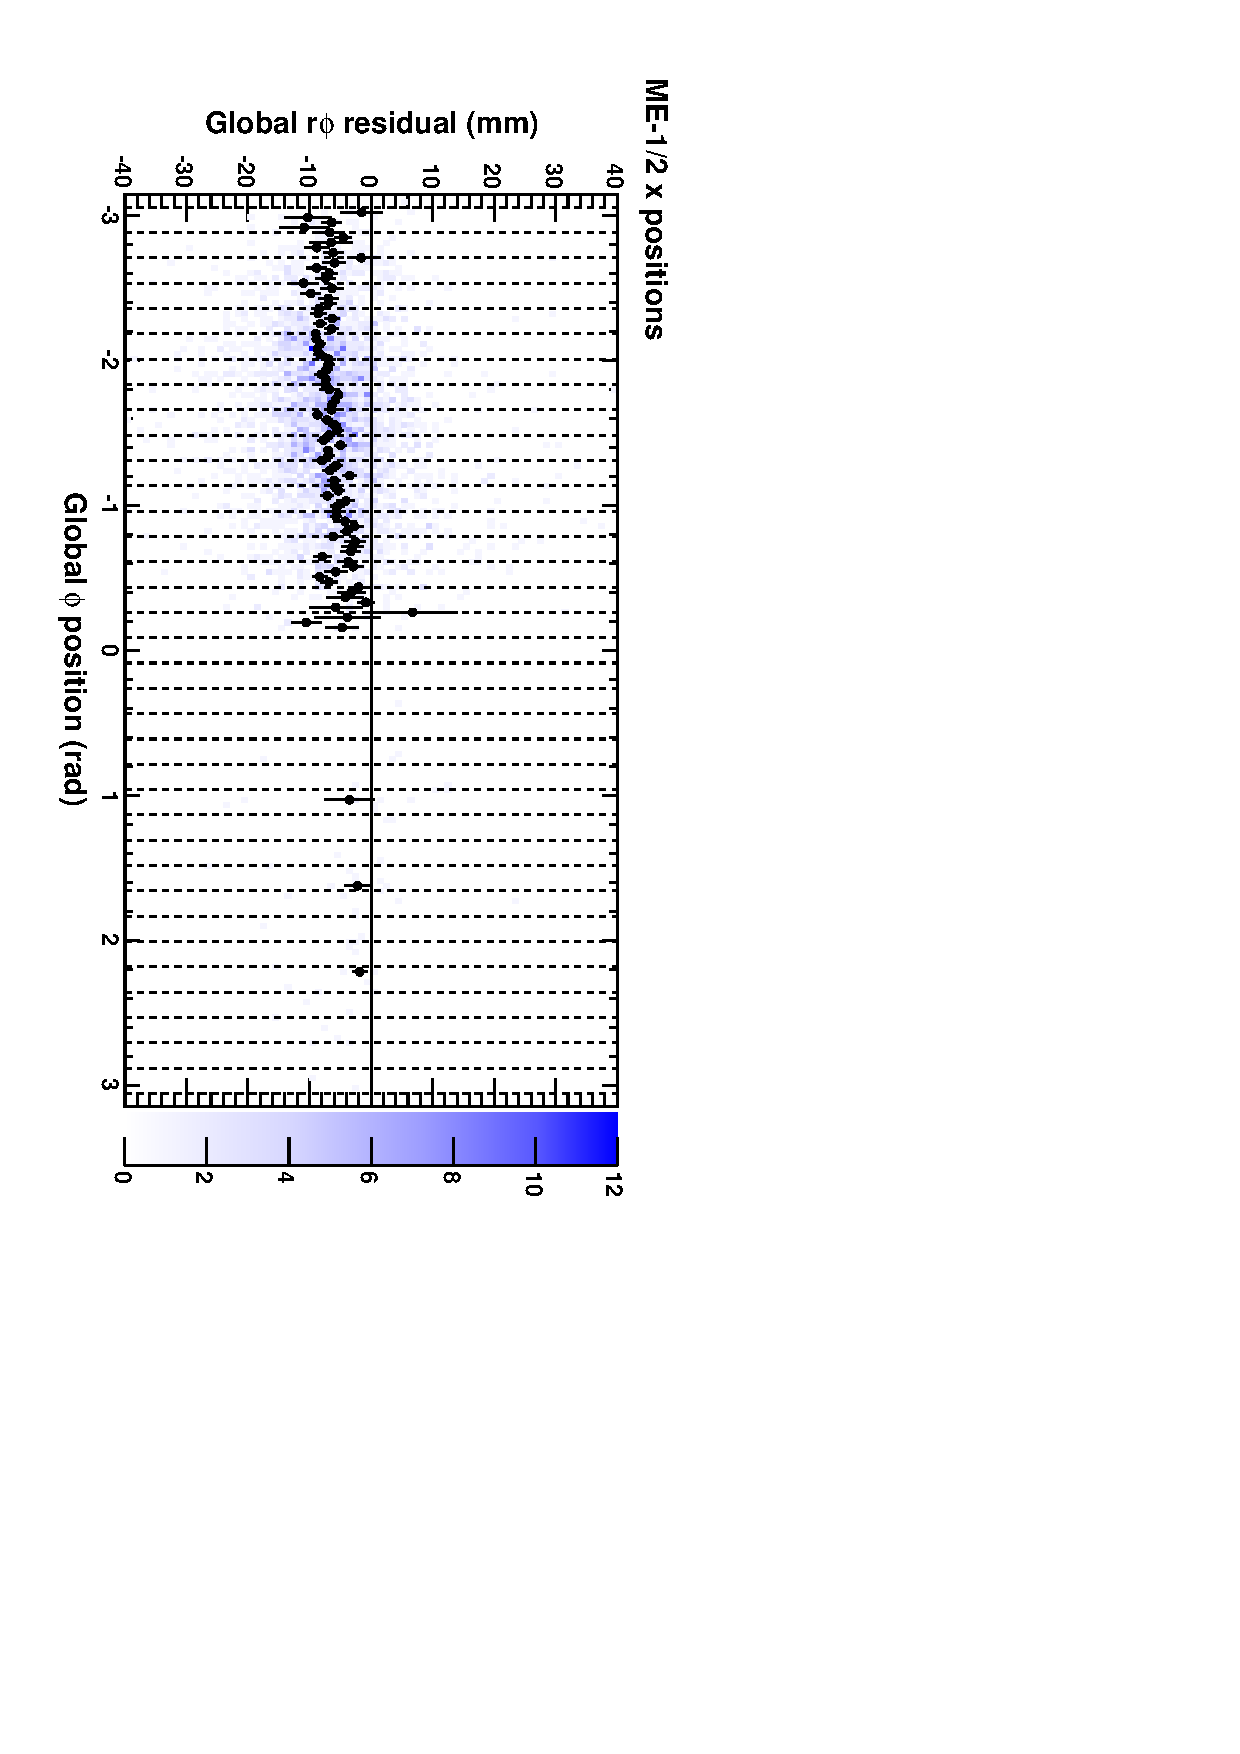
\includegraphics[height=\linewidth, angle=90]{datacsc_all_mem12x.pdf}}
\only<2>{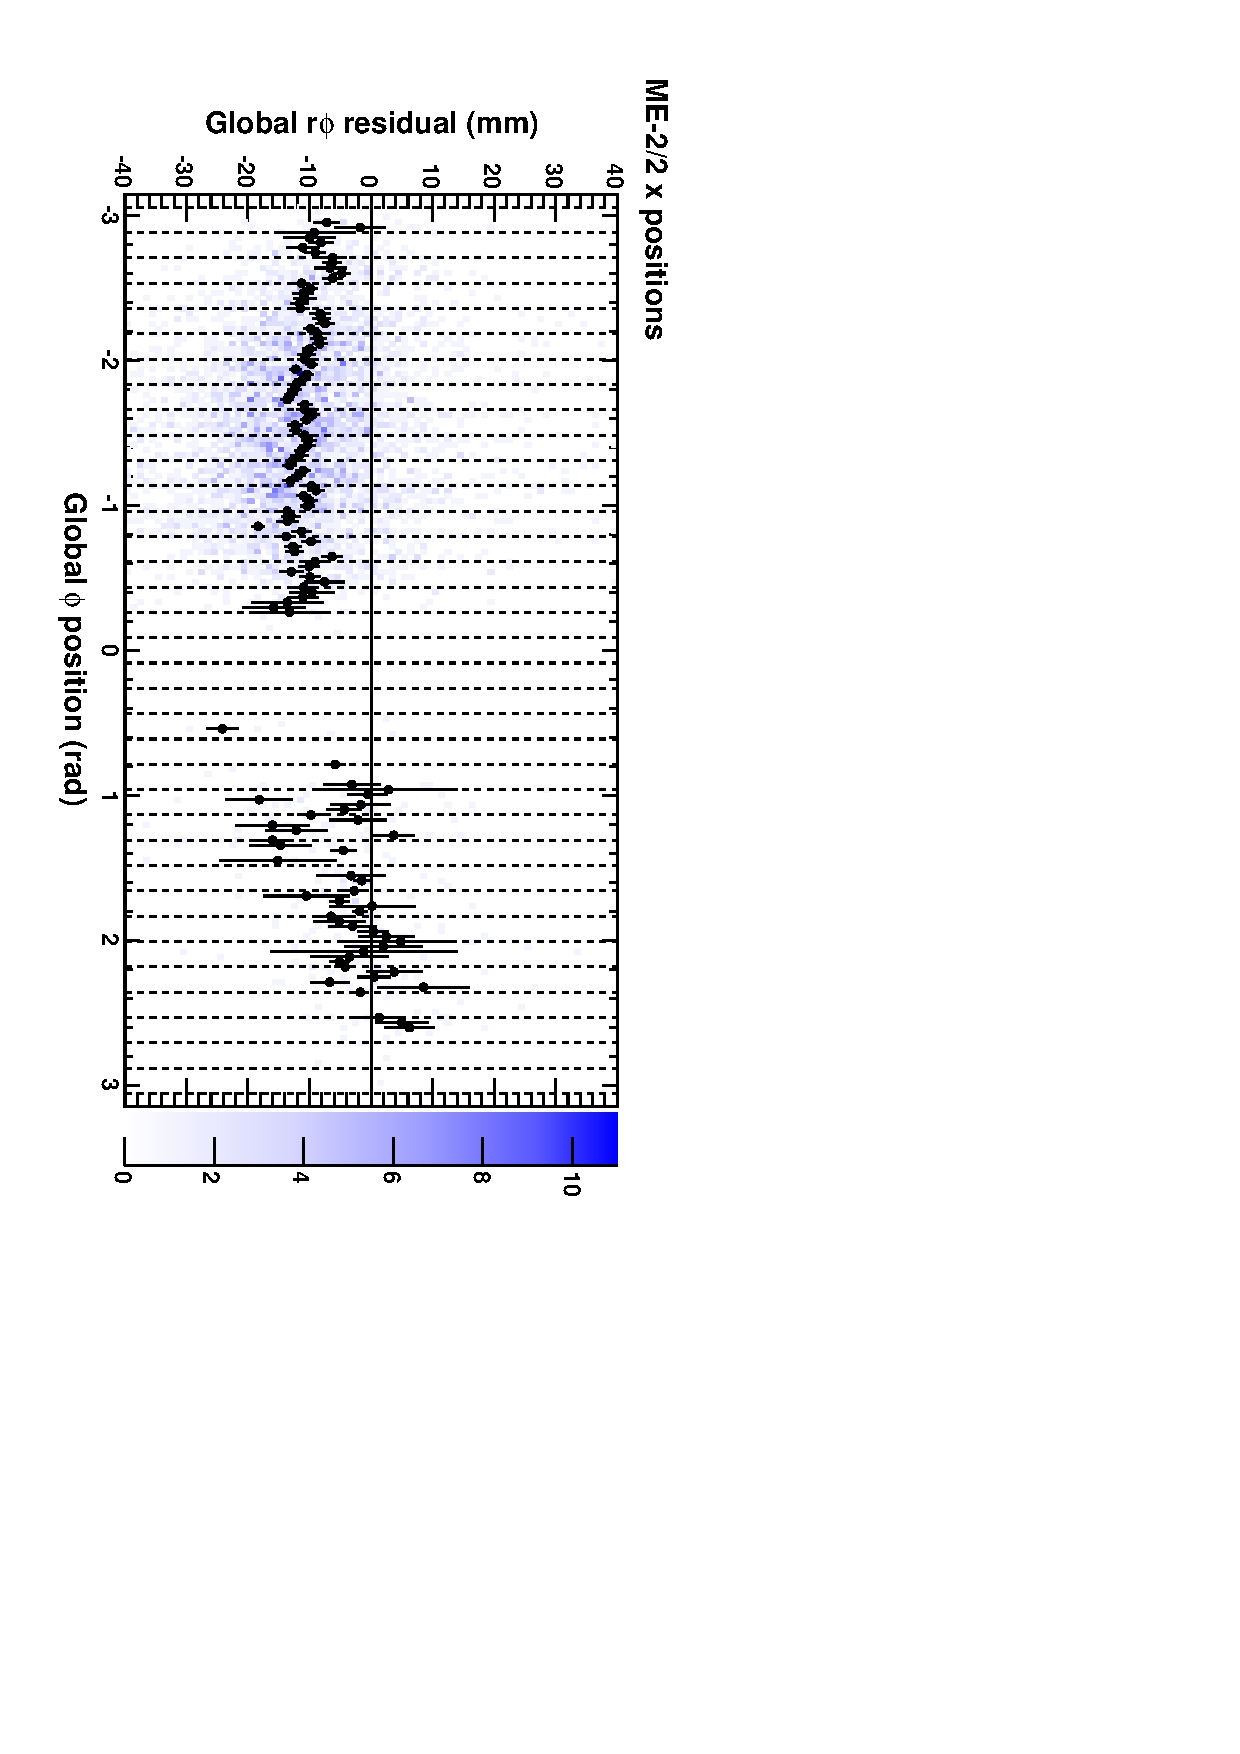
\includegraphics[height=\linewidth, angle=90]{datacsc_all_mem22x.pdf}}
\only<3>{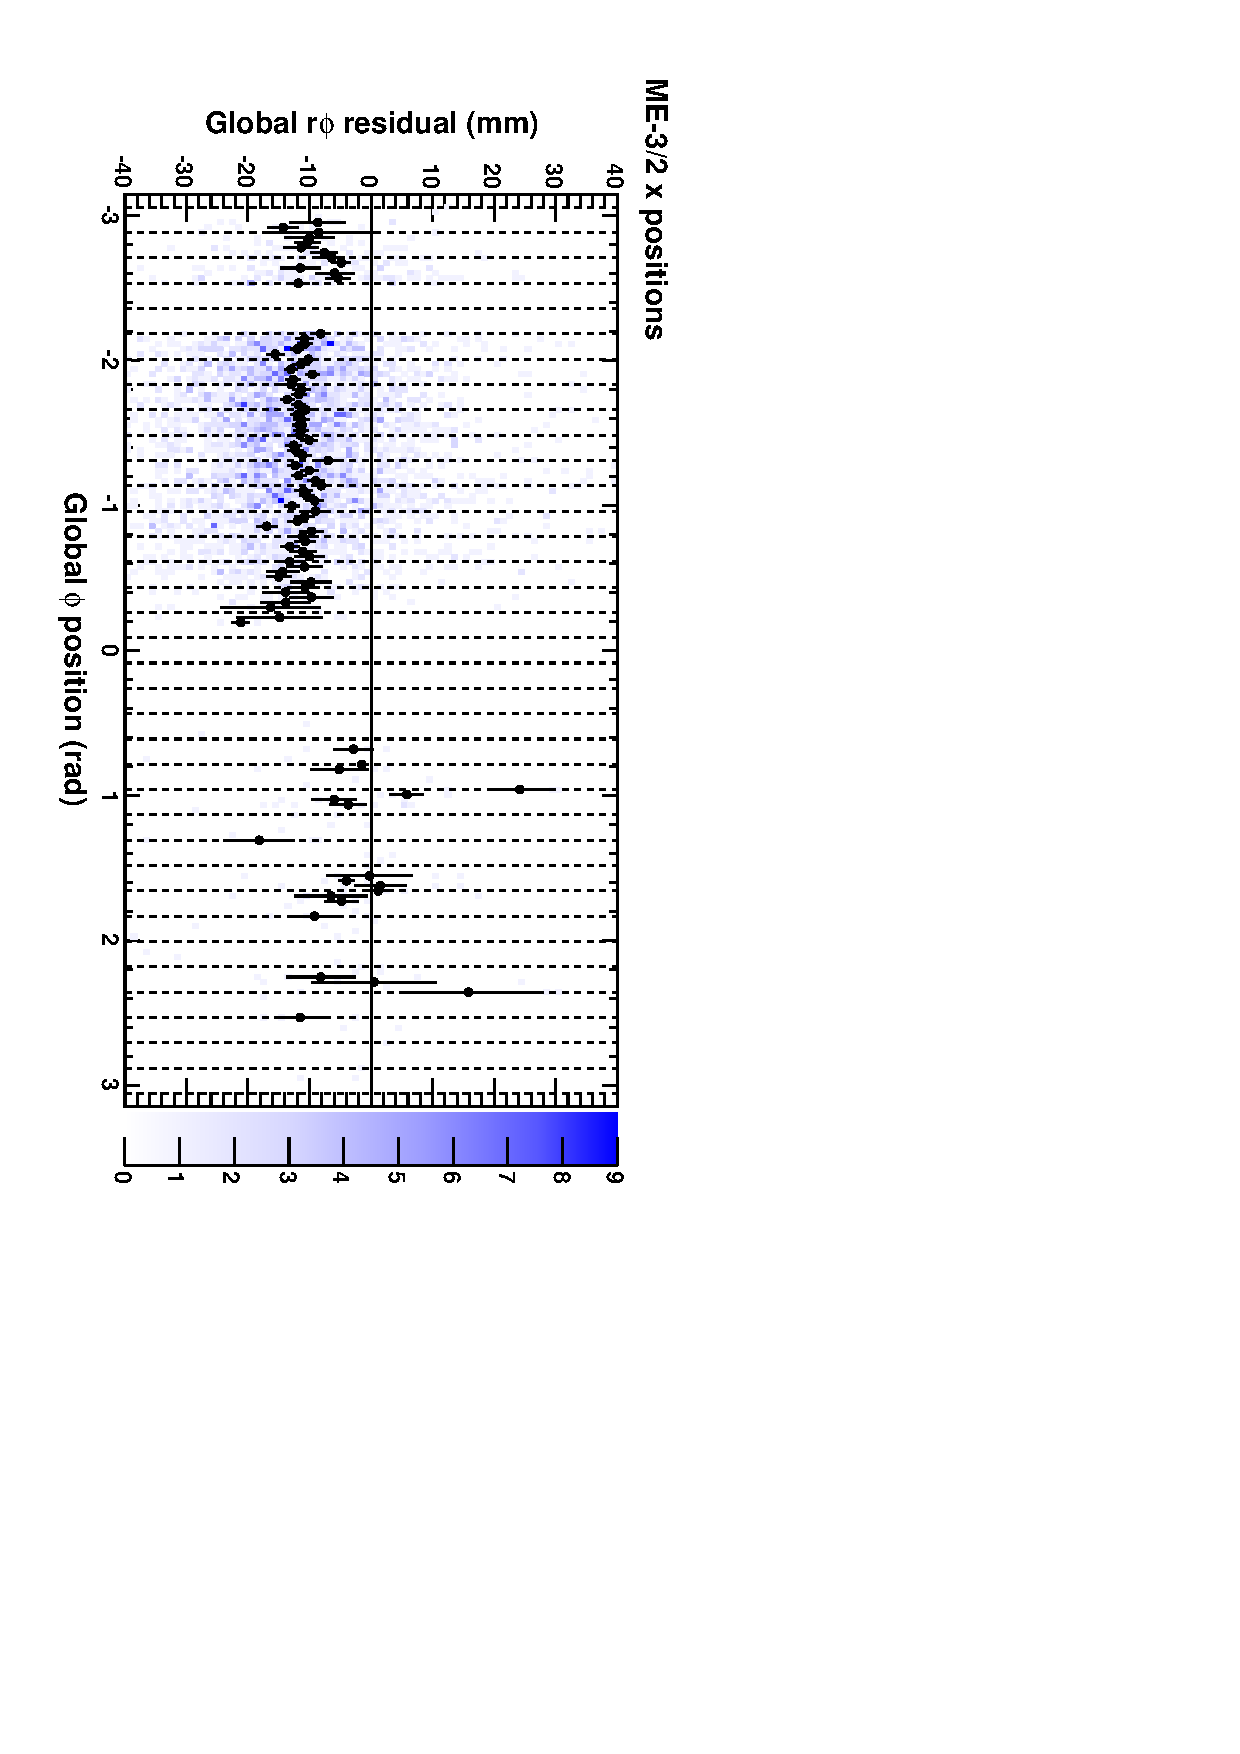
\includegraphics[height=\linewidth, angle=90]{datacsc_all_mem32x.pdf}}
\only<4>{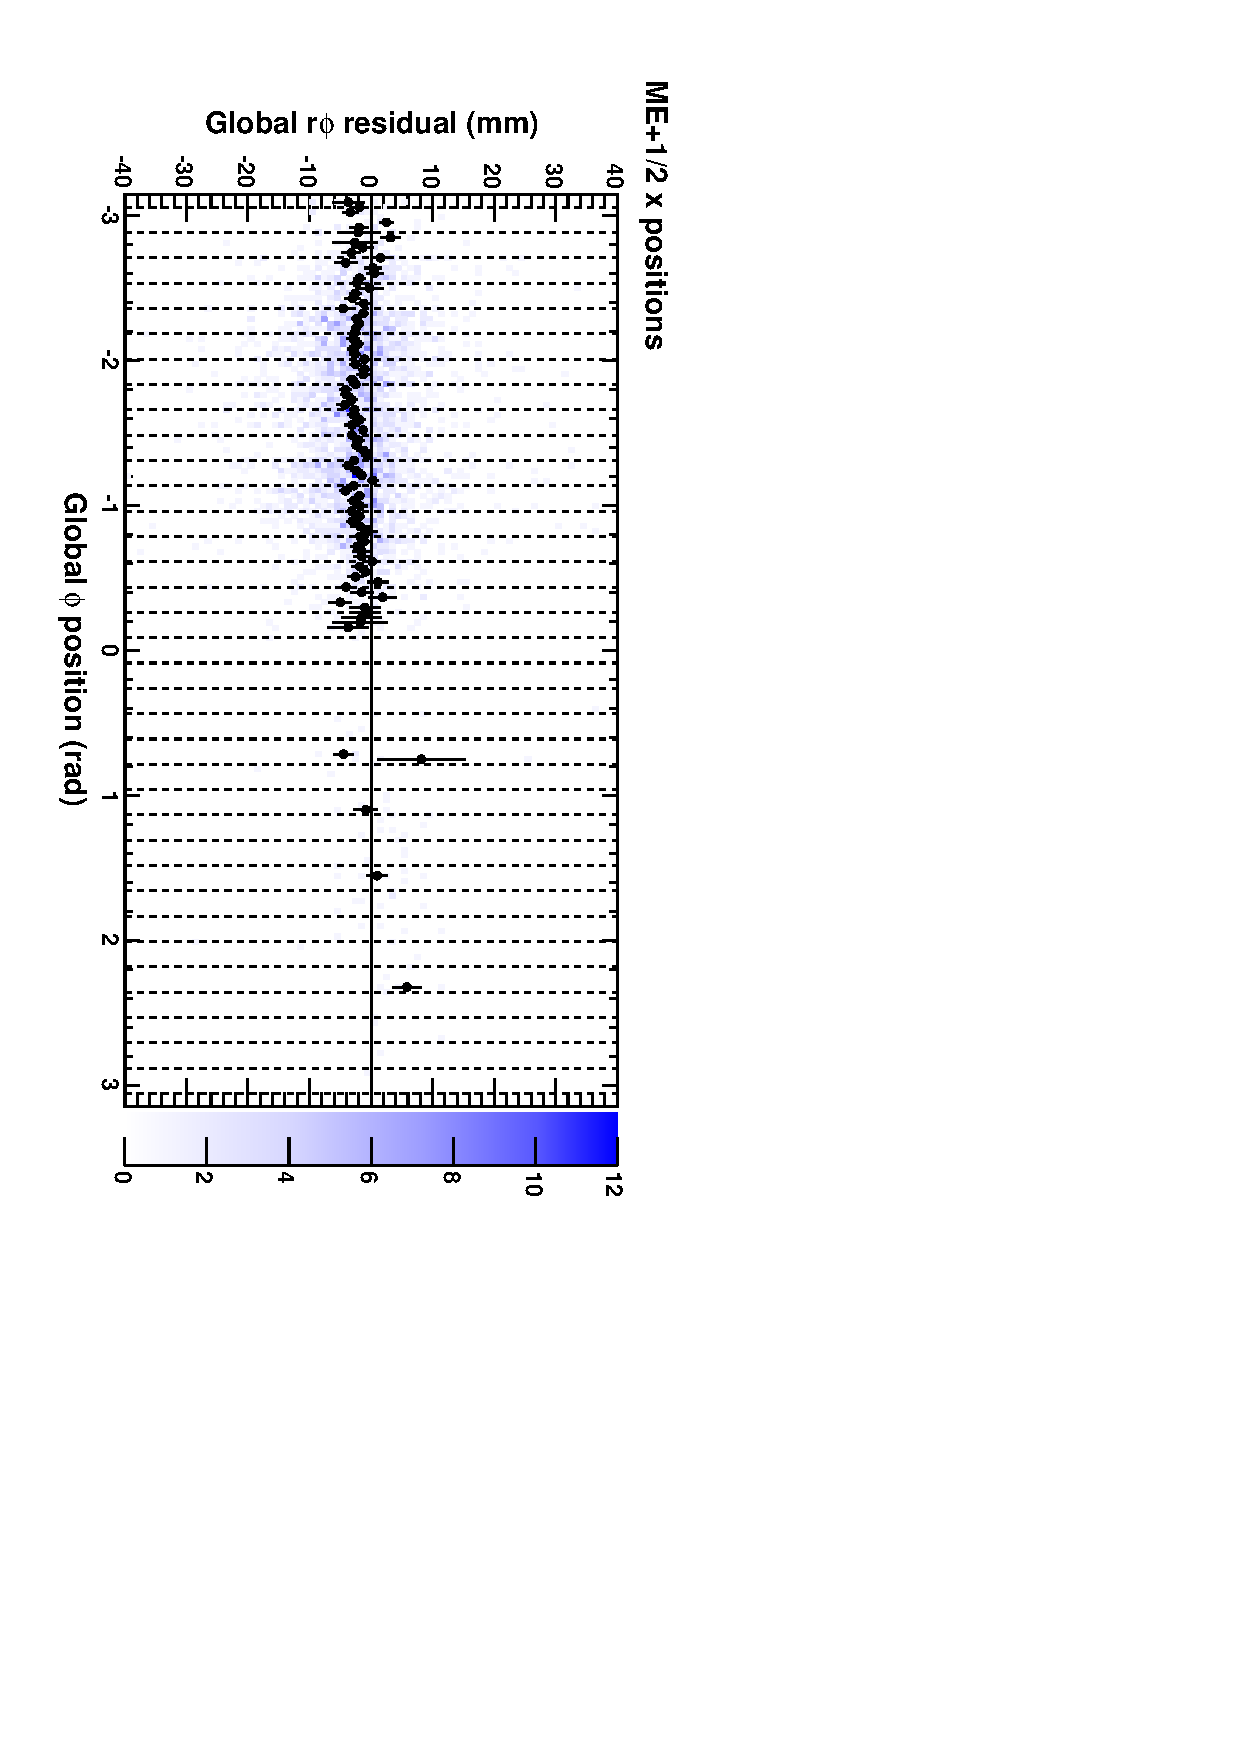
\includegraphics[height=\linewidth, angle=90]{datacsc_all_mep12x.pdf}}
\only<5>{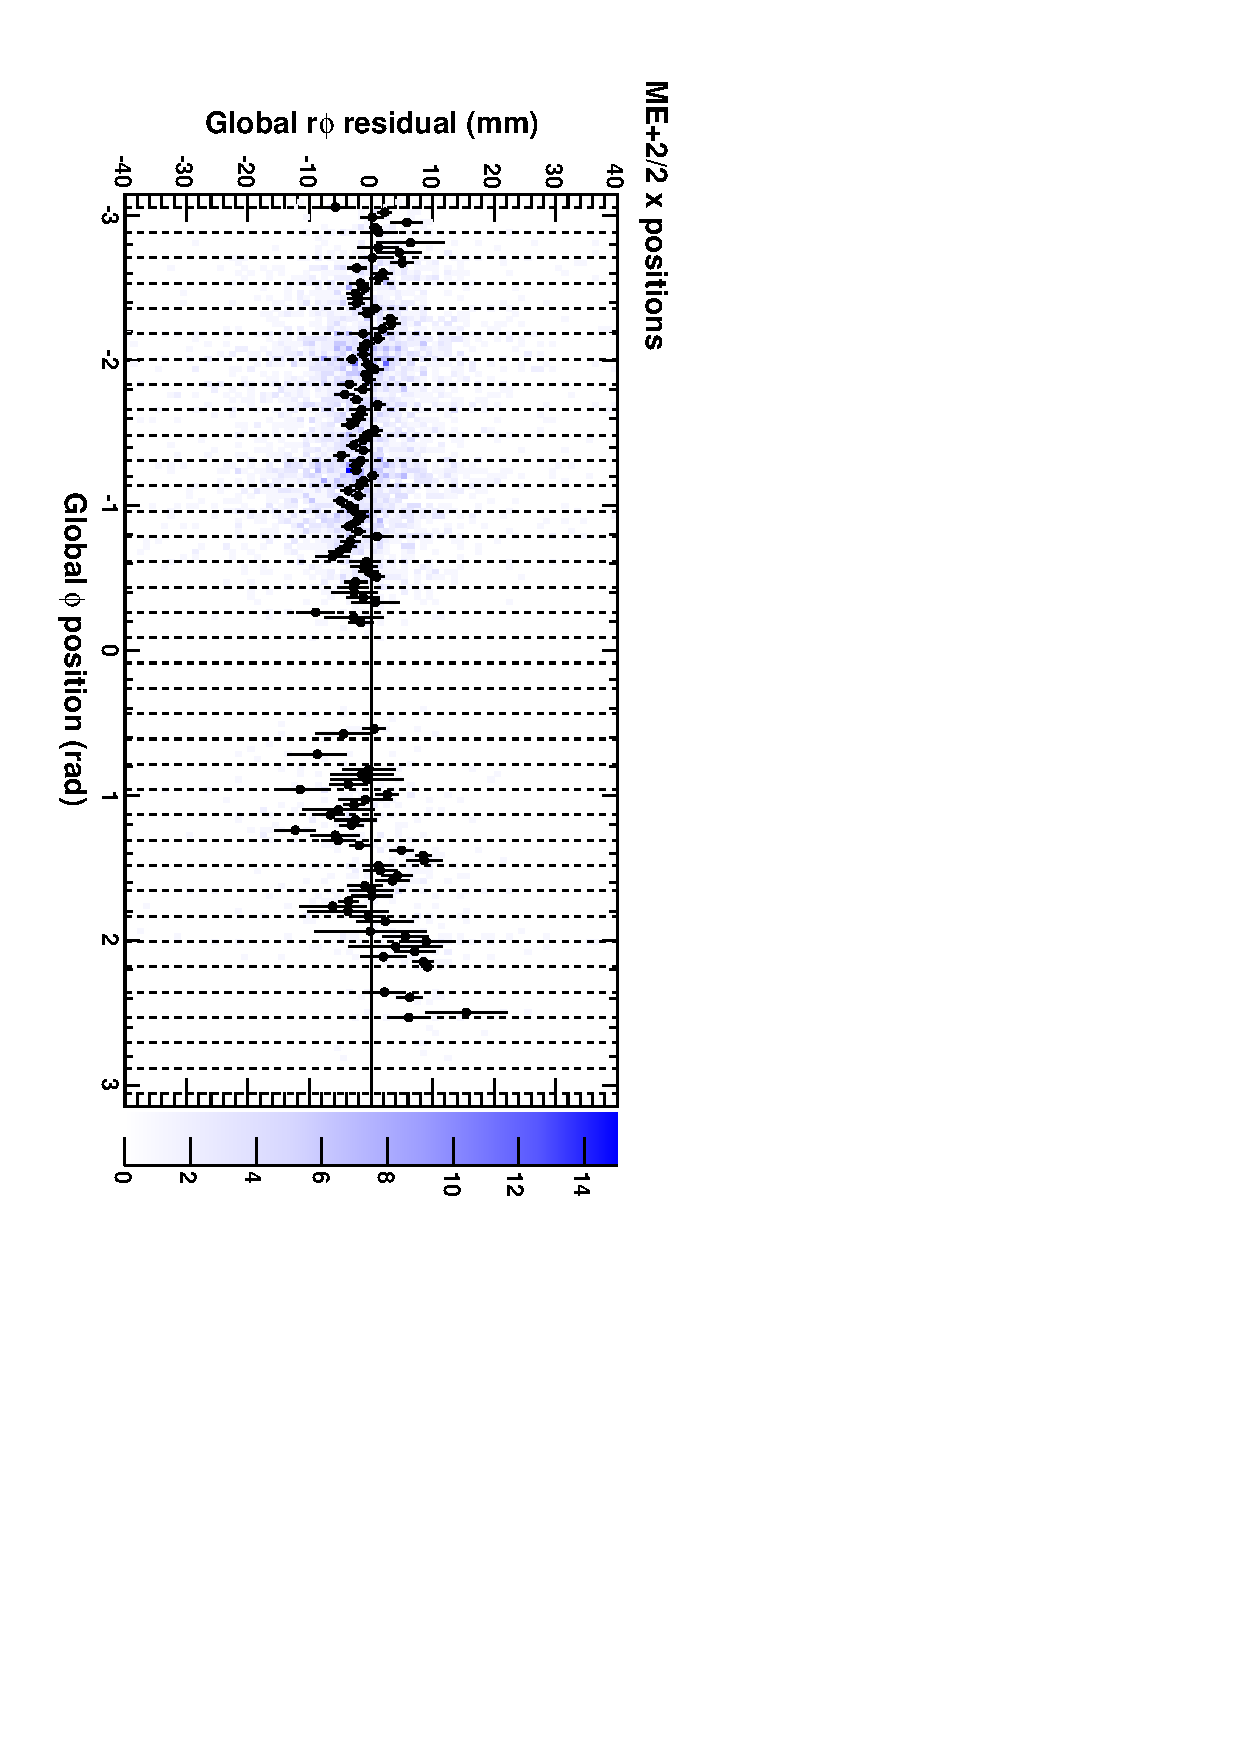
\includegraphics[height=\linewidth, angle=90]{datacsc_all_mep22x.pdf}}
\only<6>{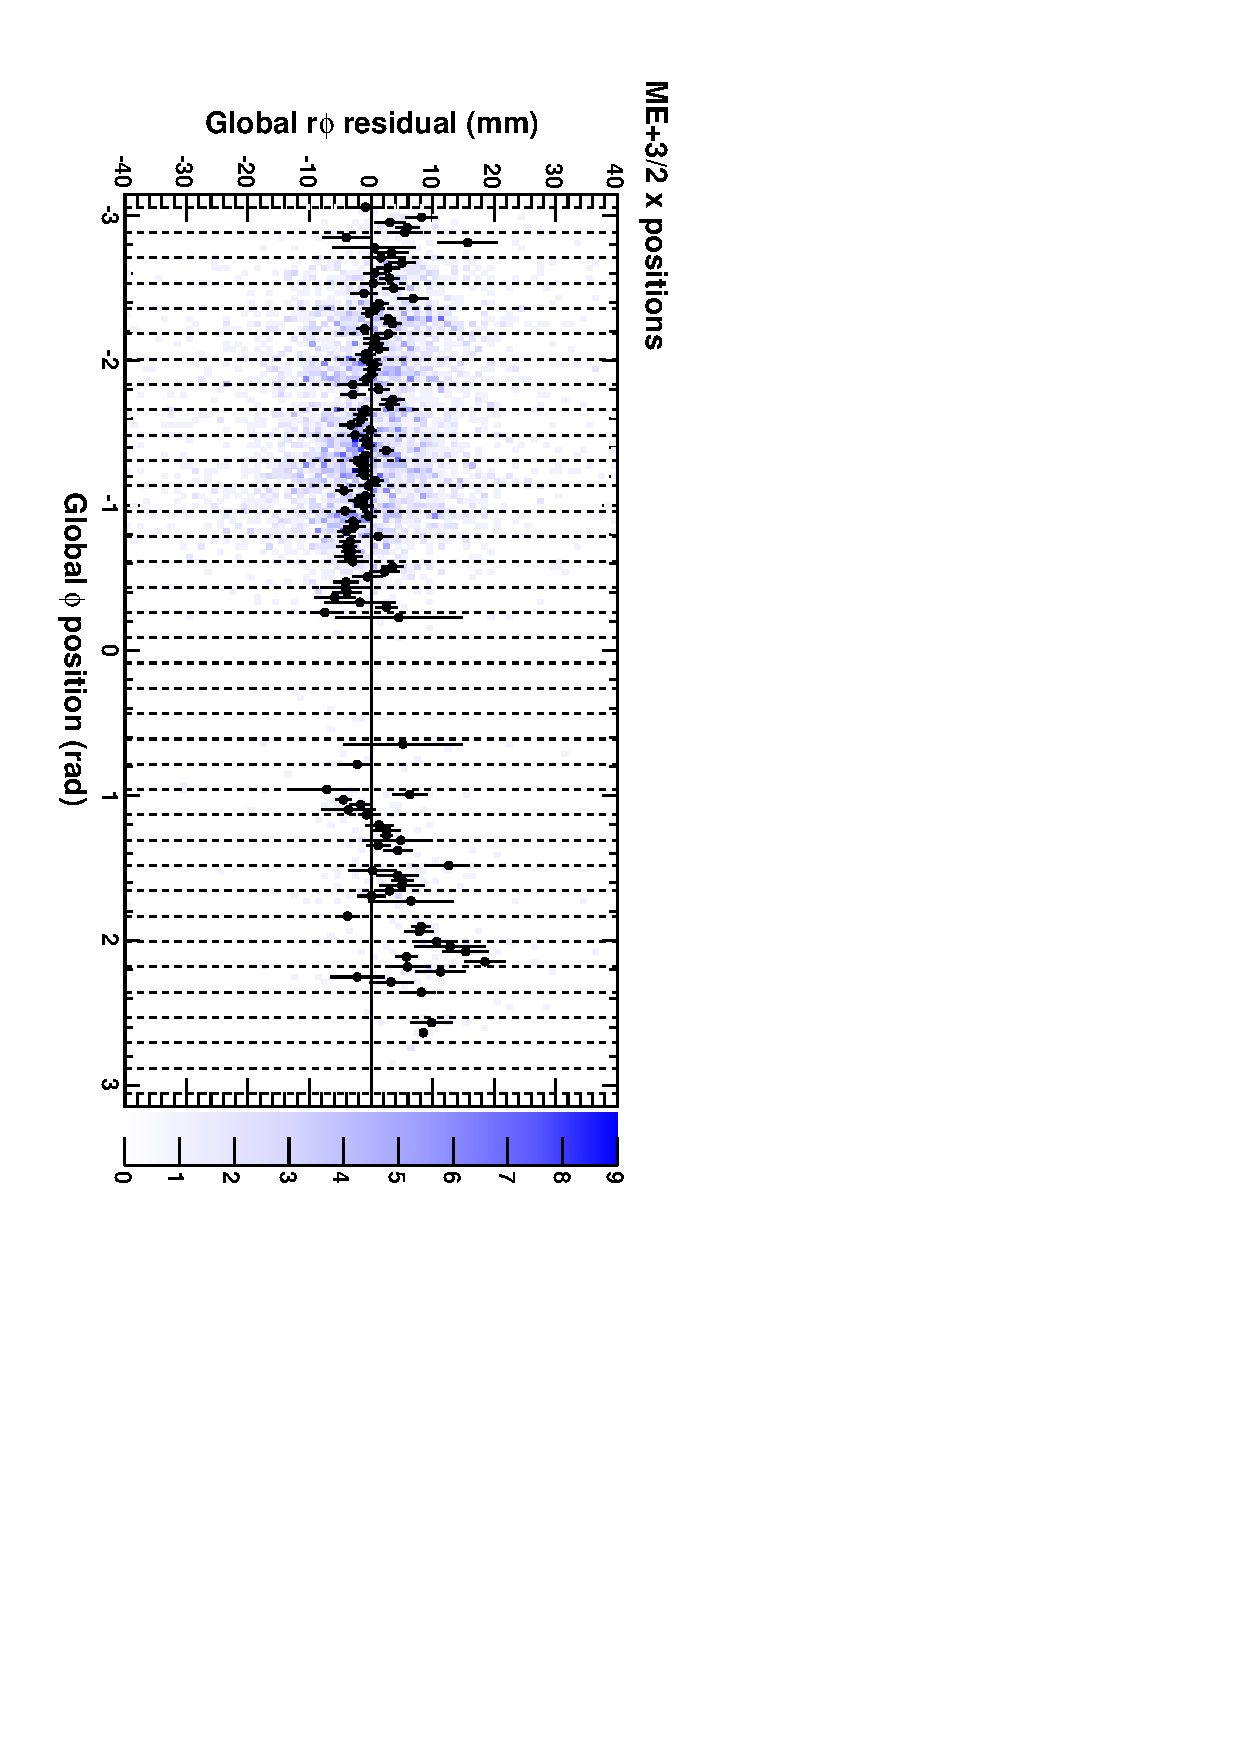
\includegraphics[height=\linewidth, angle=90]{datacsc_all_mep32x.pdf}}
\only<7>{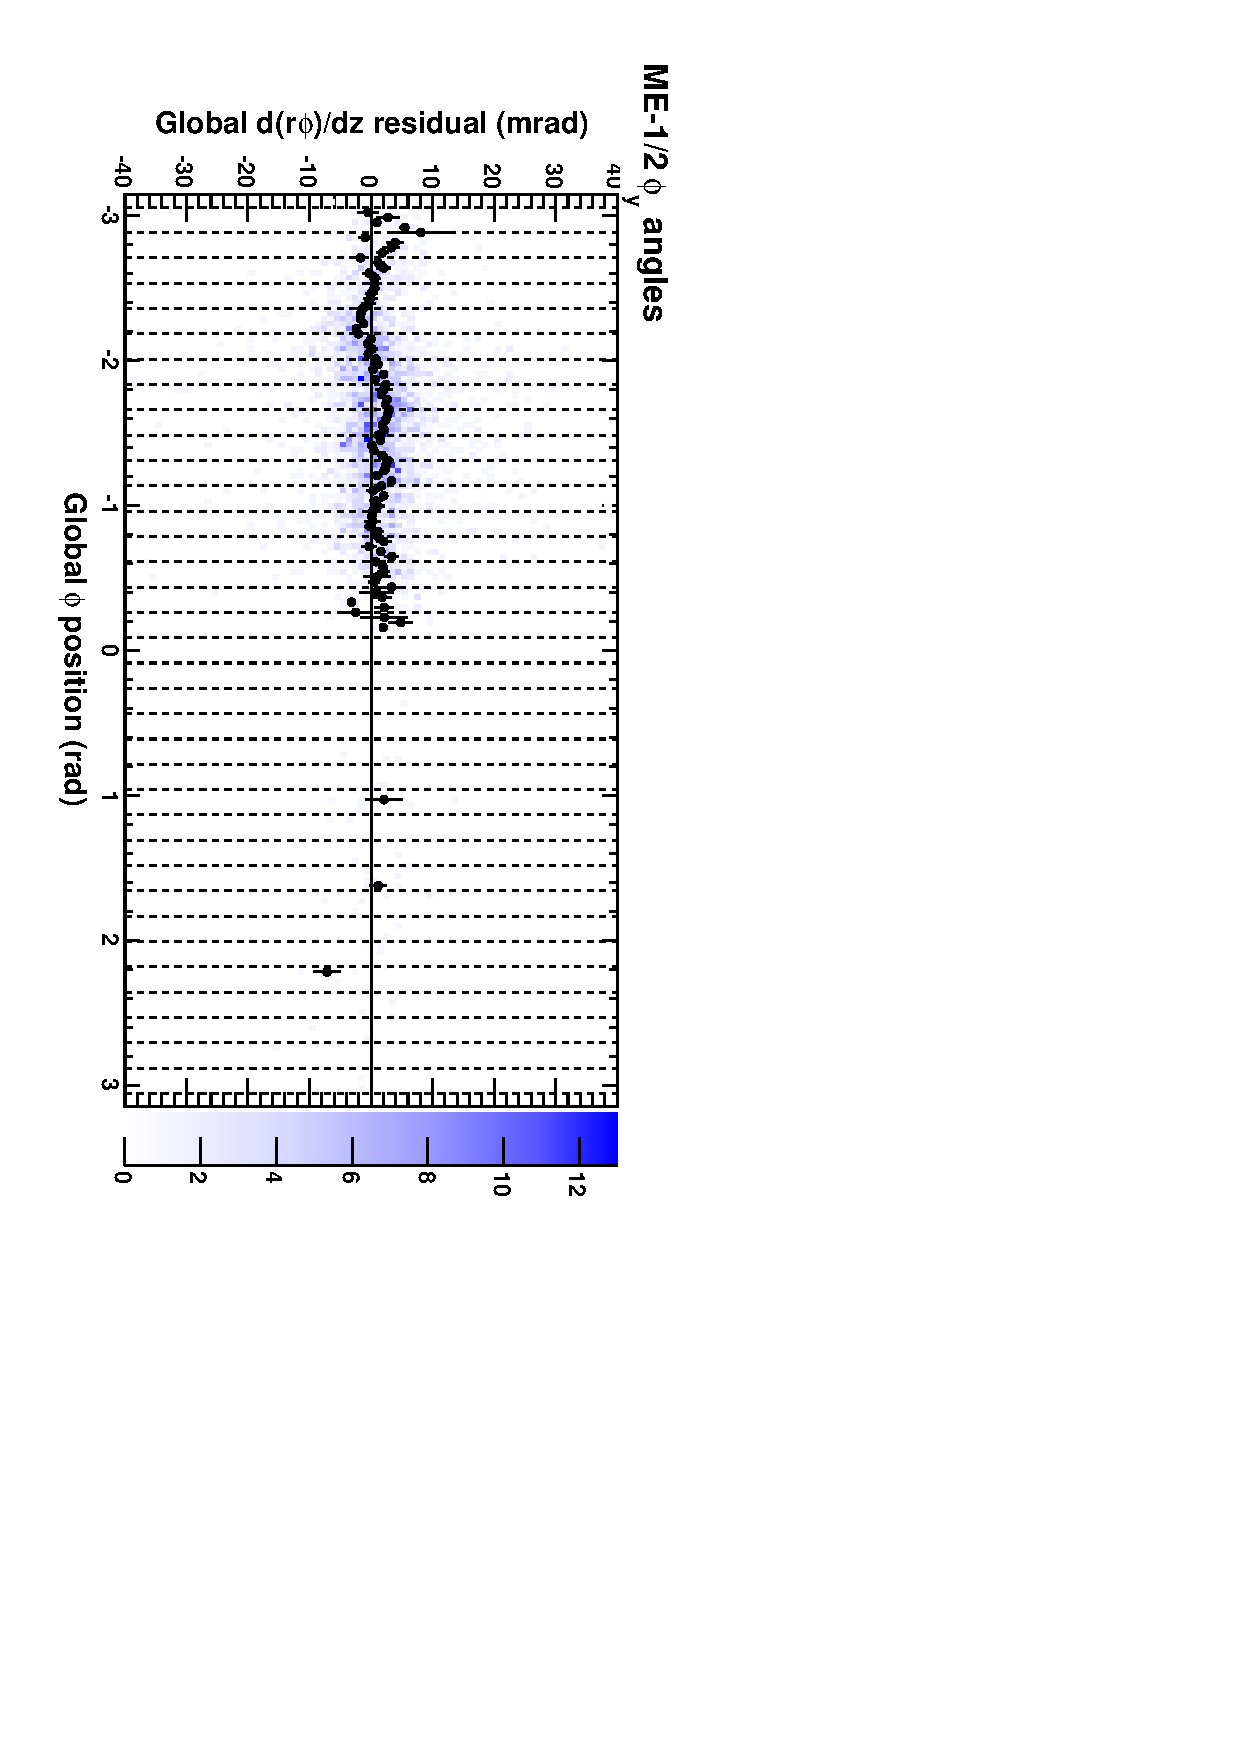
\includegraphics[height=\linewidth, angle=90]{datacsc_all_mem12phiy.pdf}}
\only<8>{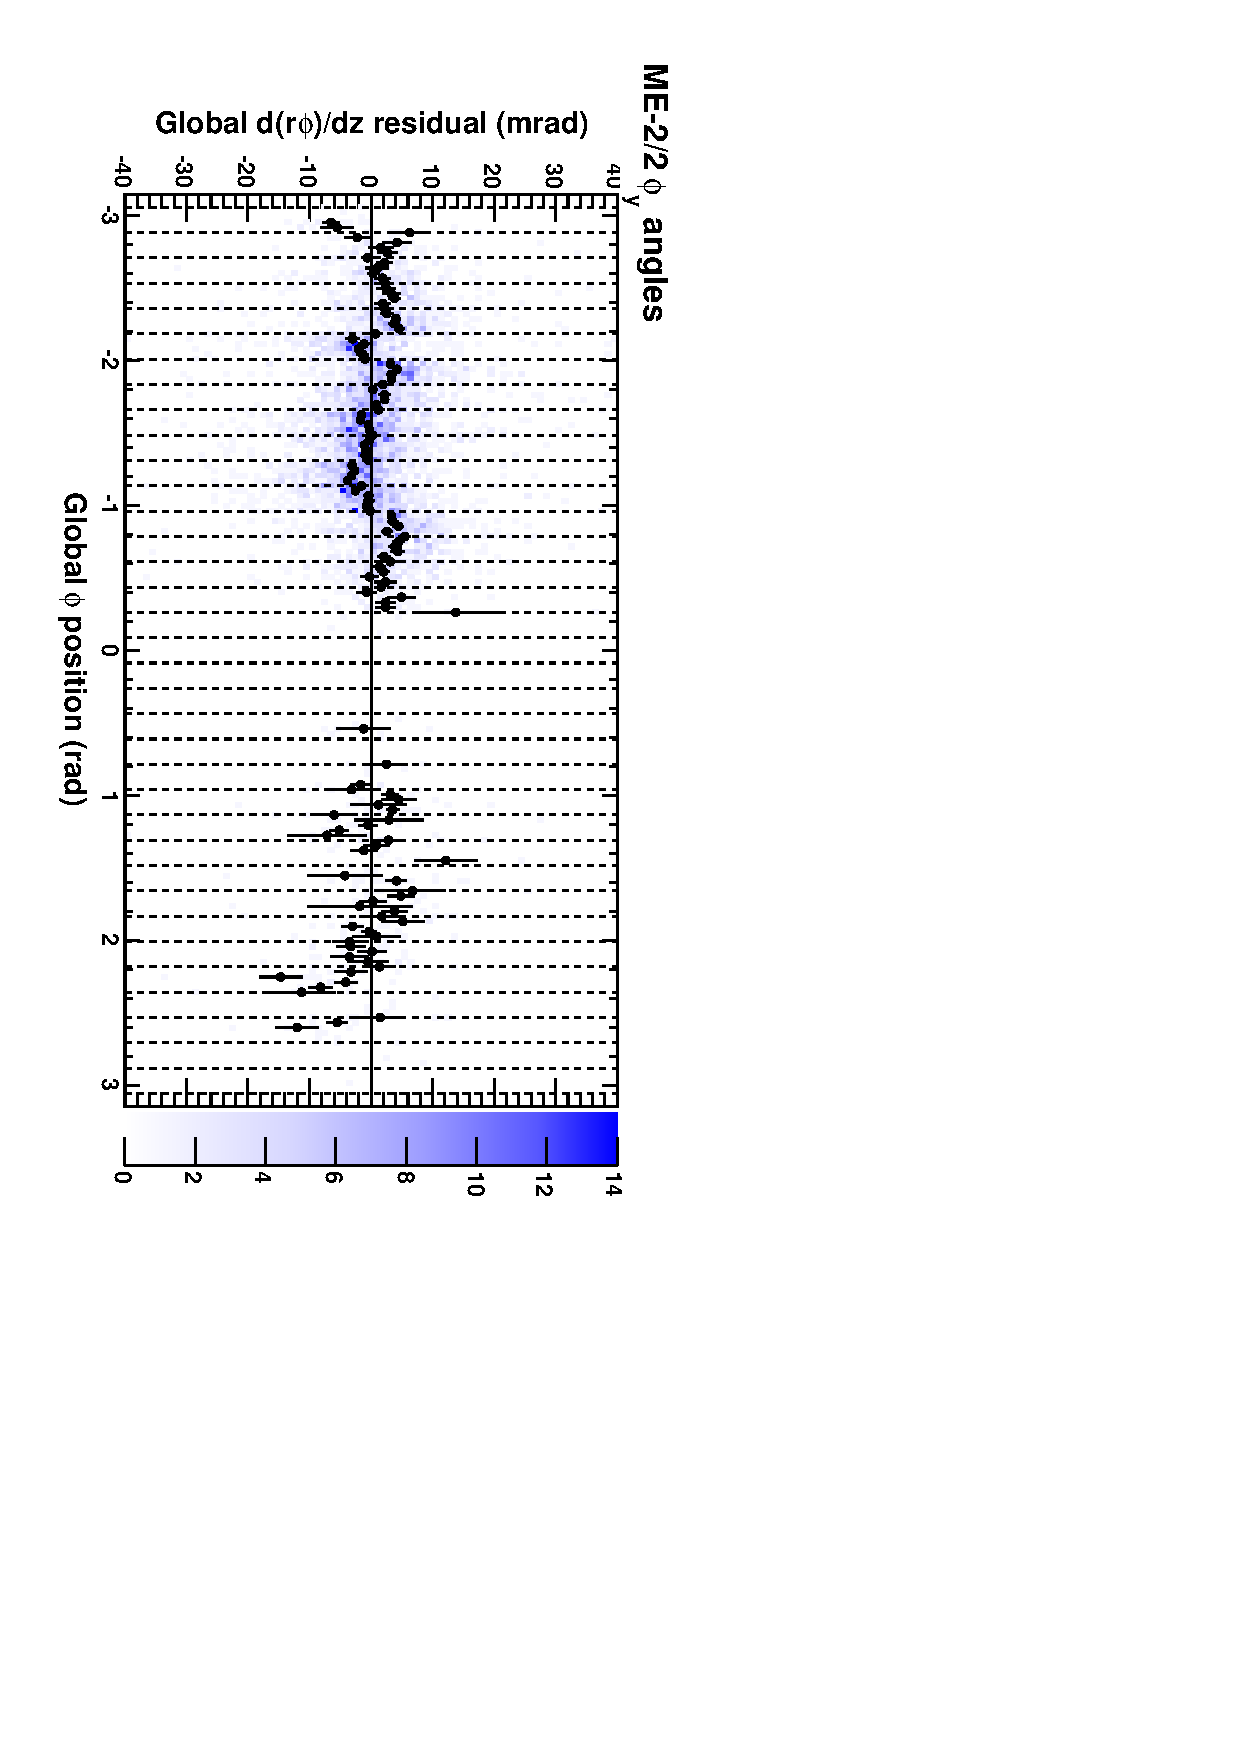
\includegraphics[height=\linewidth, angle=90]{datacsc_all_mem22phiy.pdf}}
\only<9>{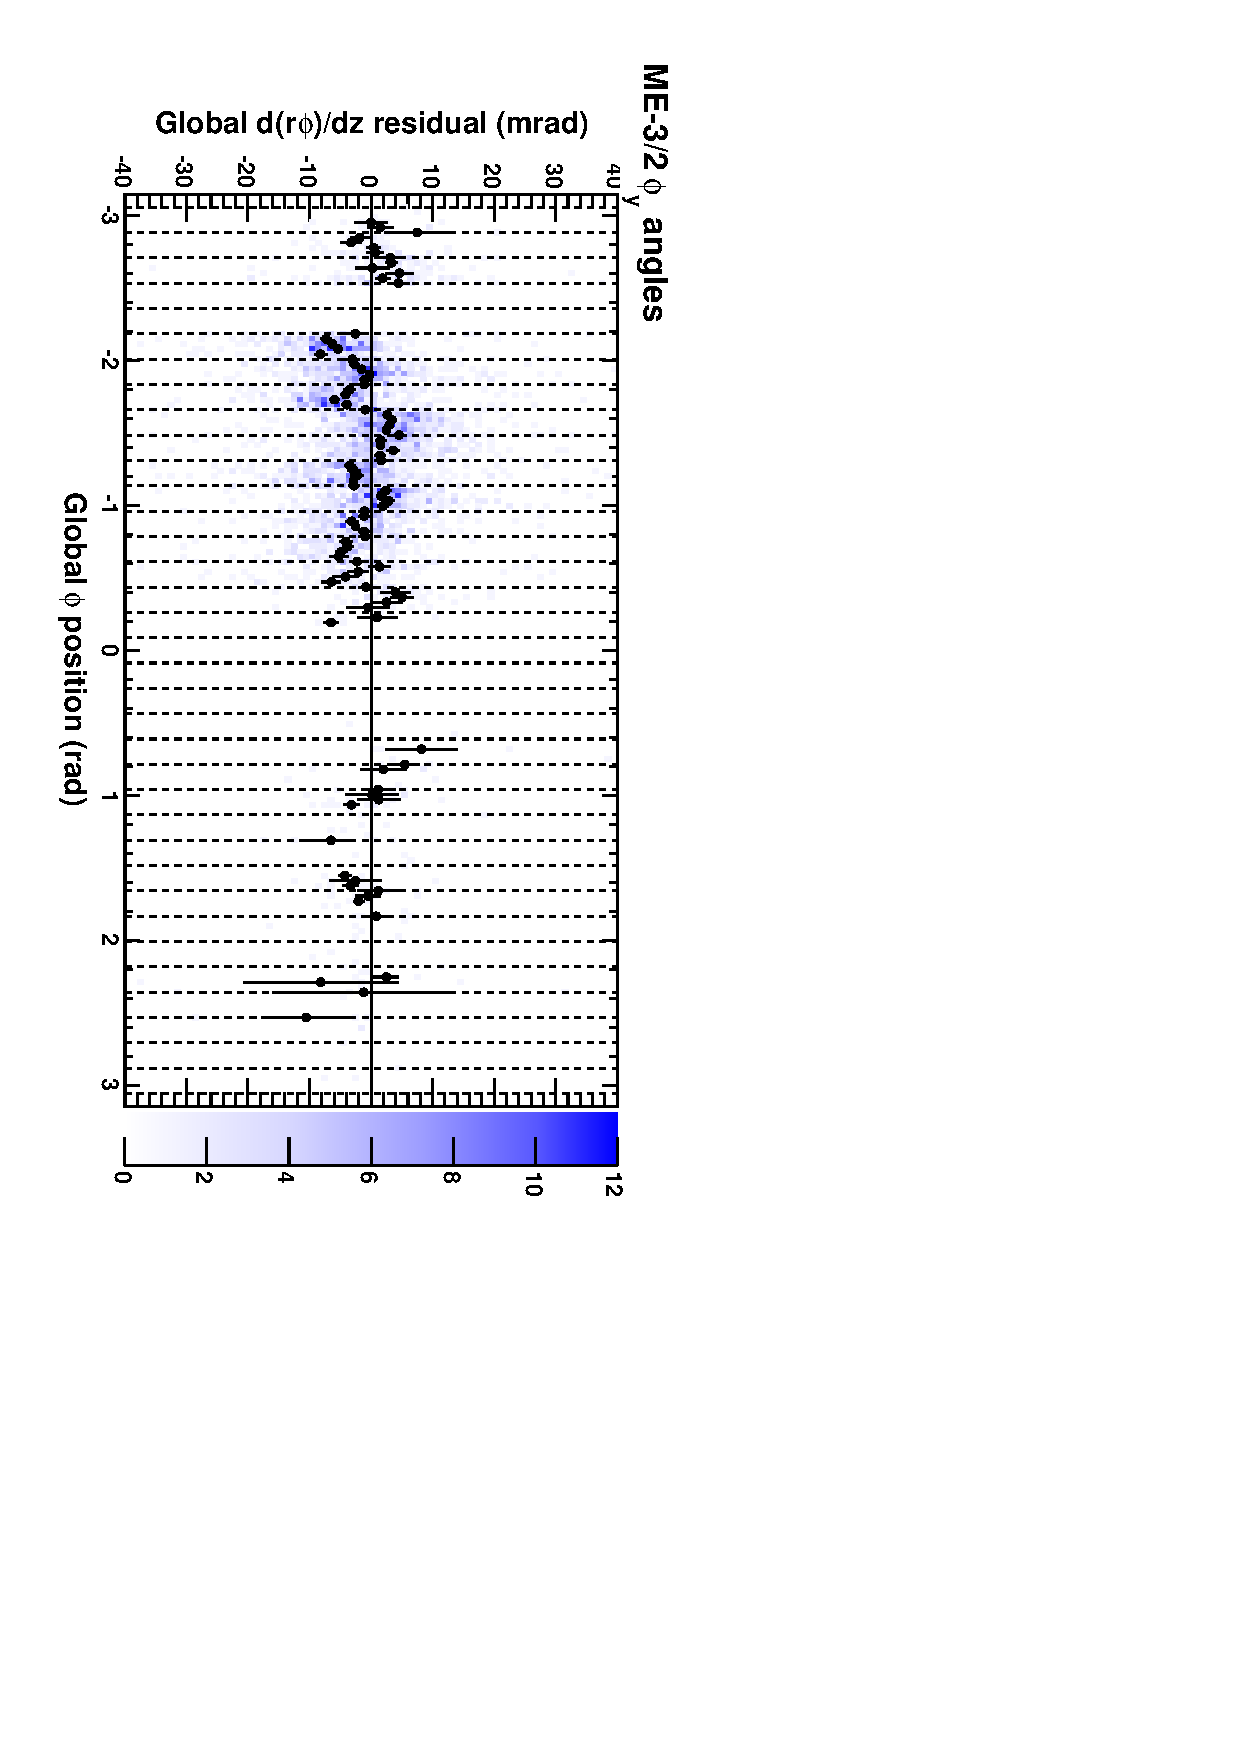
\includegraphics[height=\linewidth, angle=90]{datacsc_all_mem32phiy.pdf}}
\only<10>{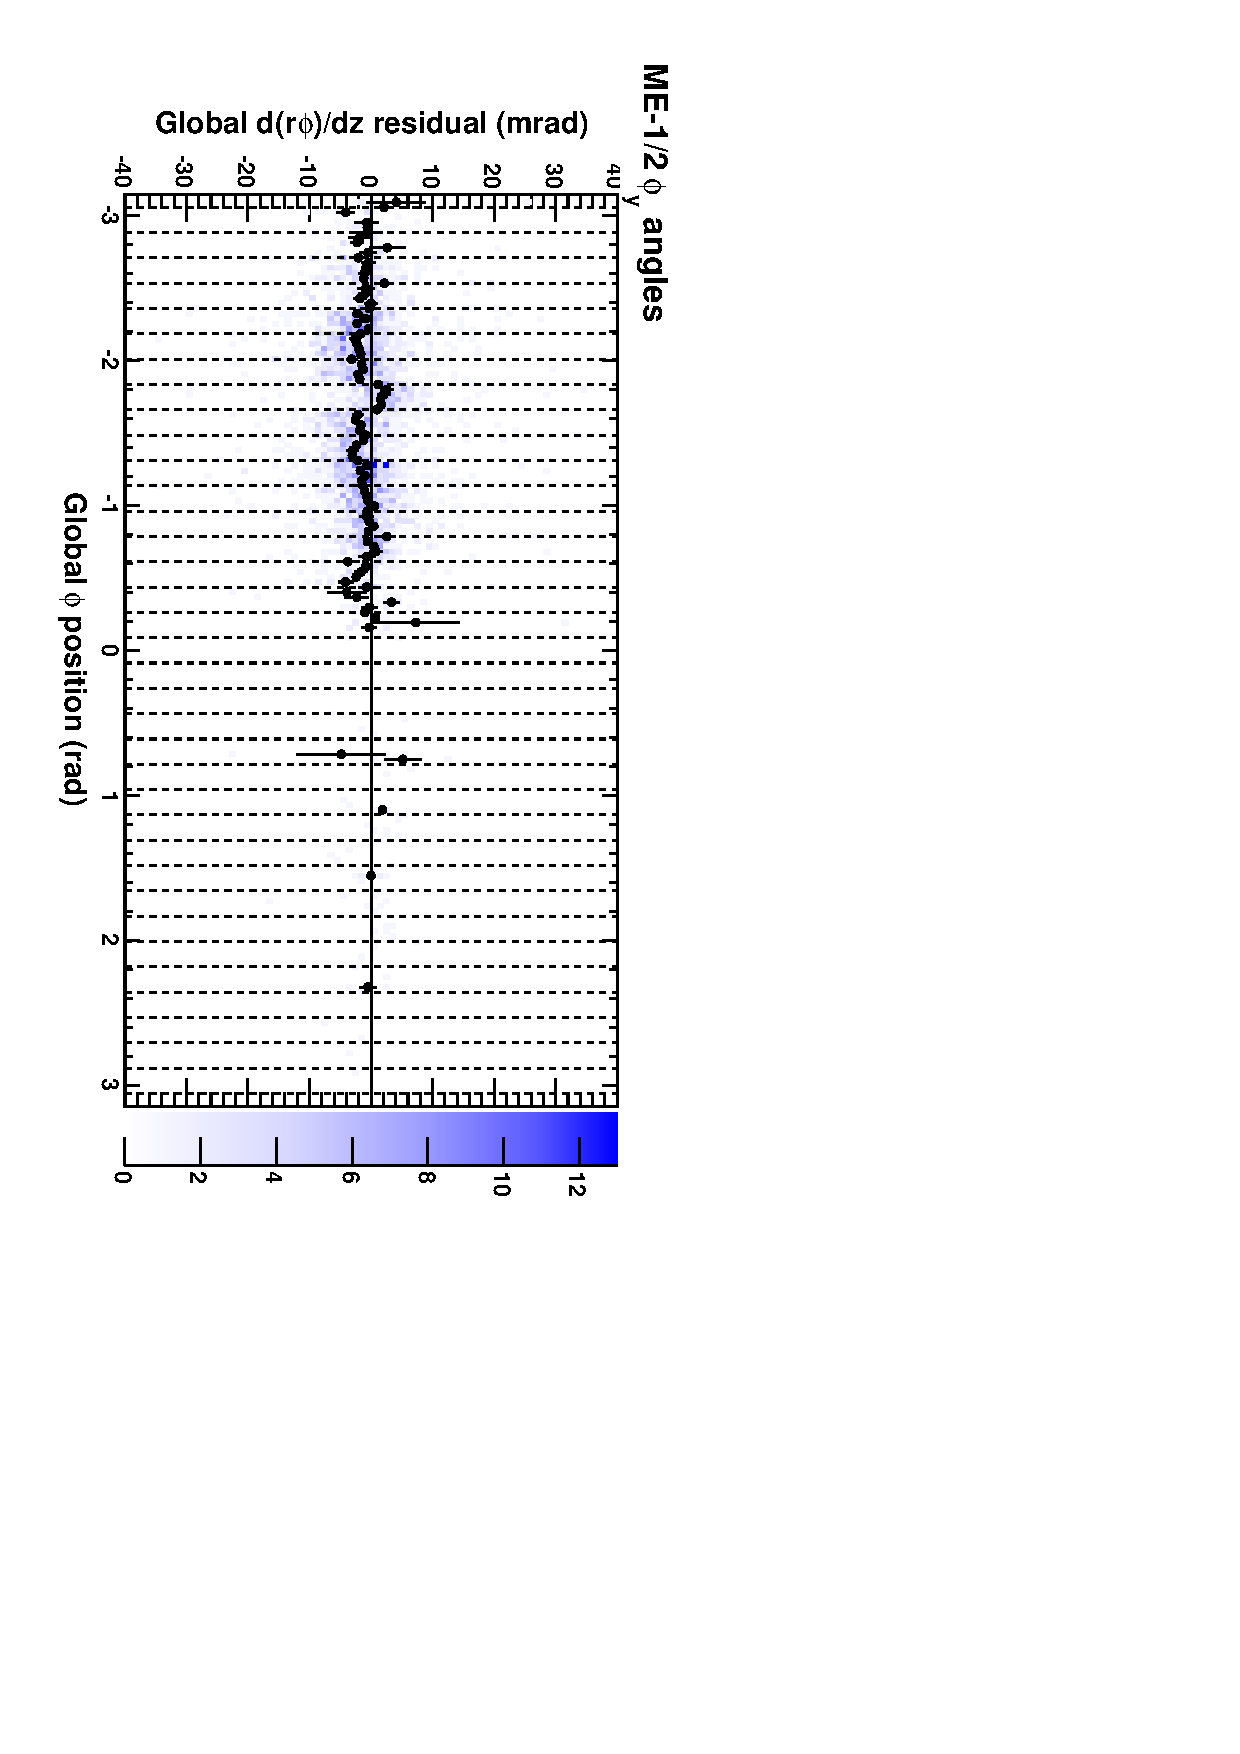
\includegraphics[height=\linewidth, angle=90]{datacsc_all_mep12phiy.pdf}}
\only<11>{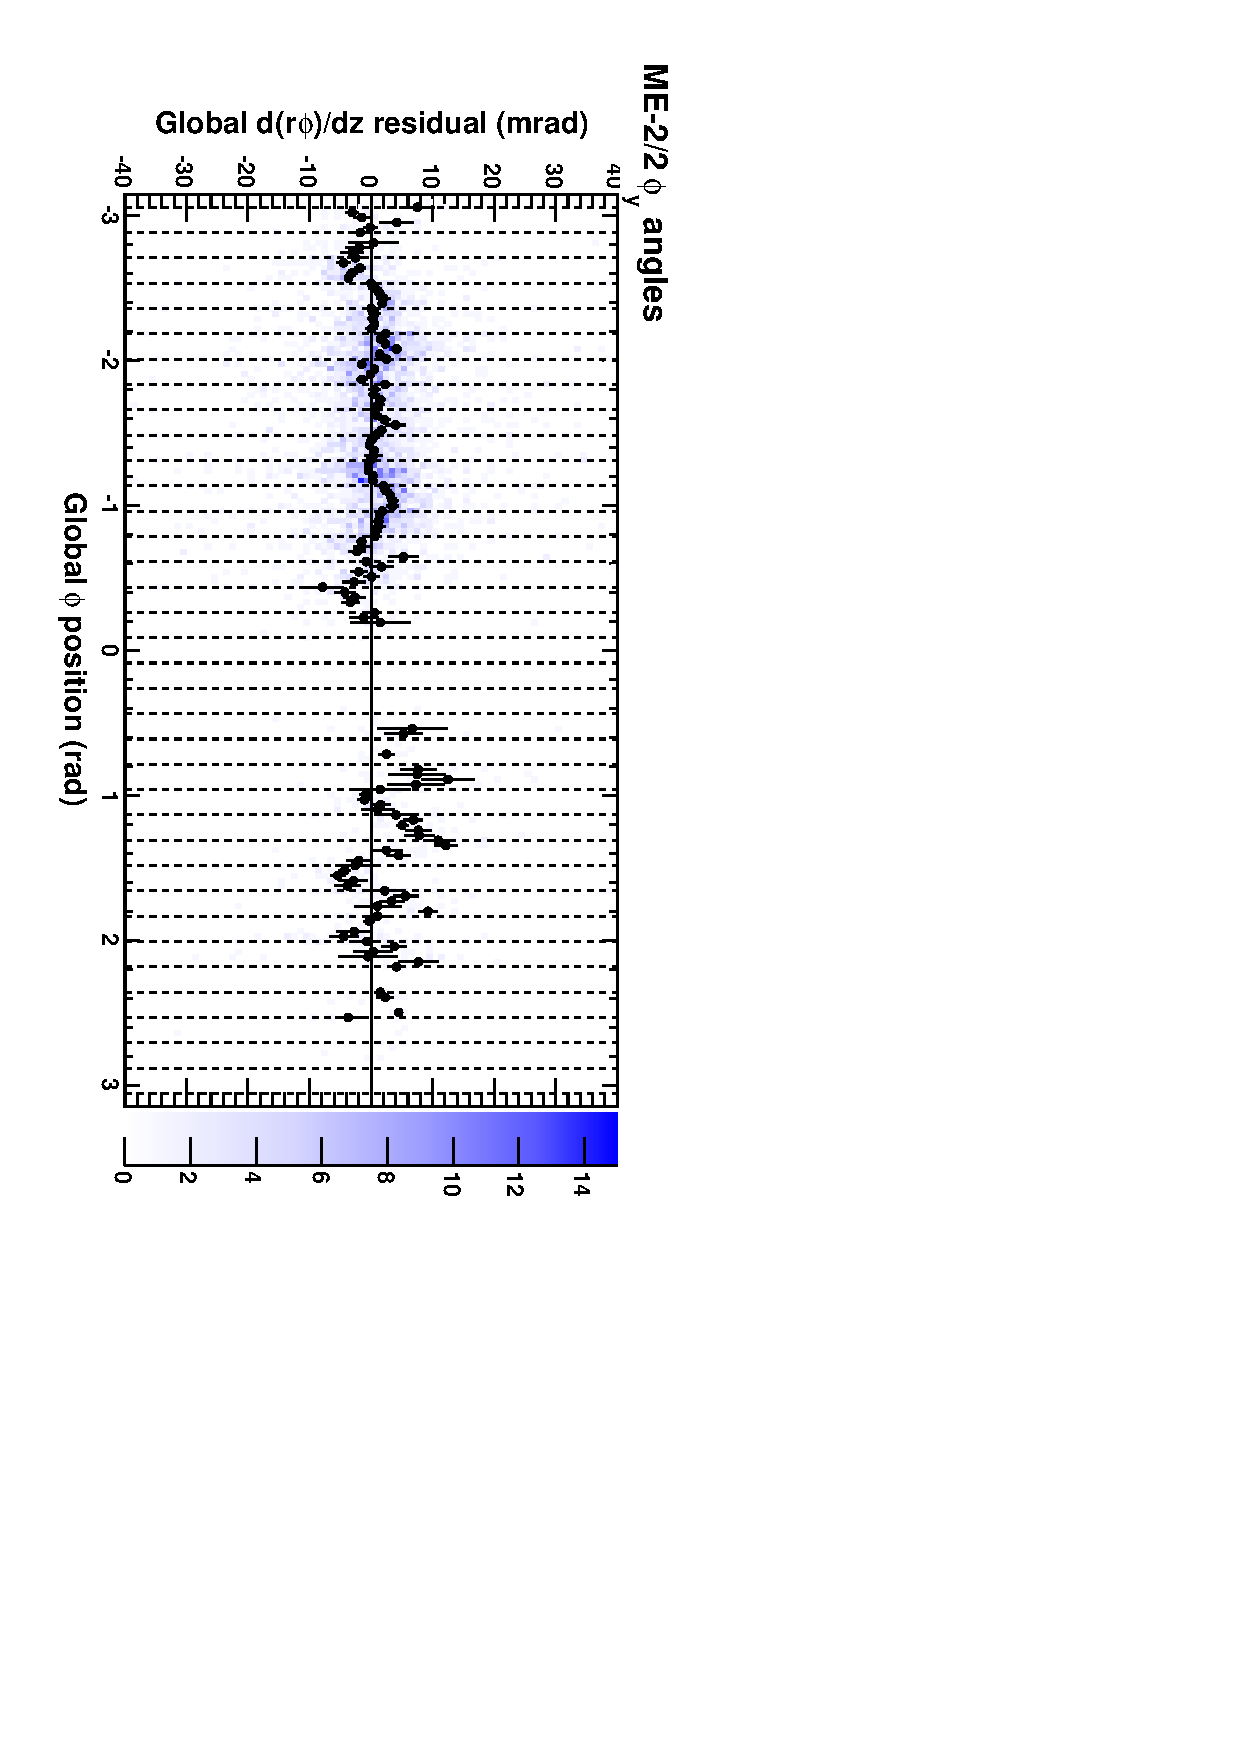
\includegraphics[height=\linewidth, angle=90]{datacsc_all_mep22phiy.pdf}}
\only<12>{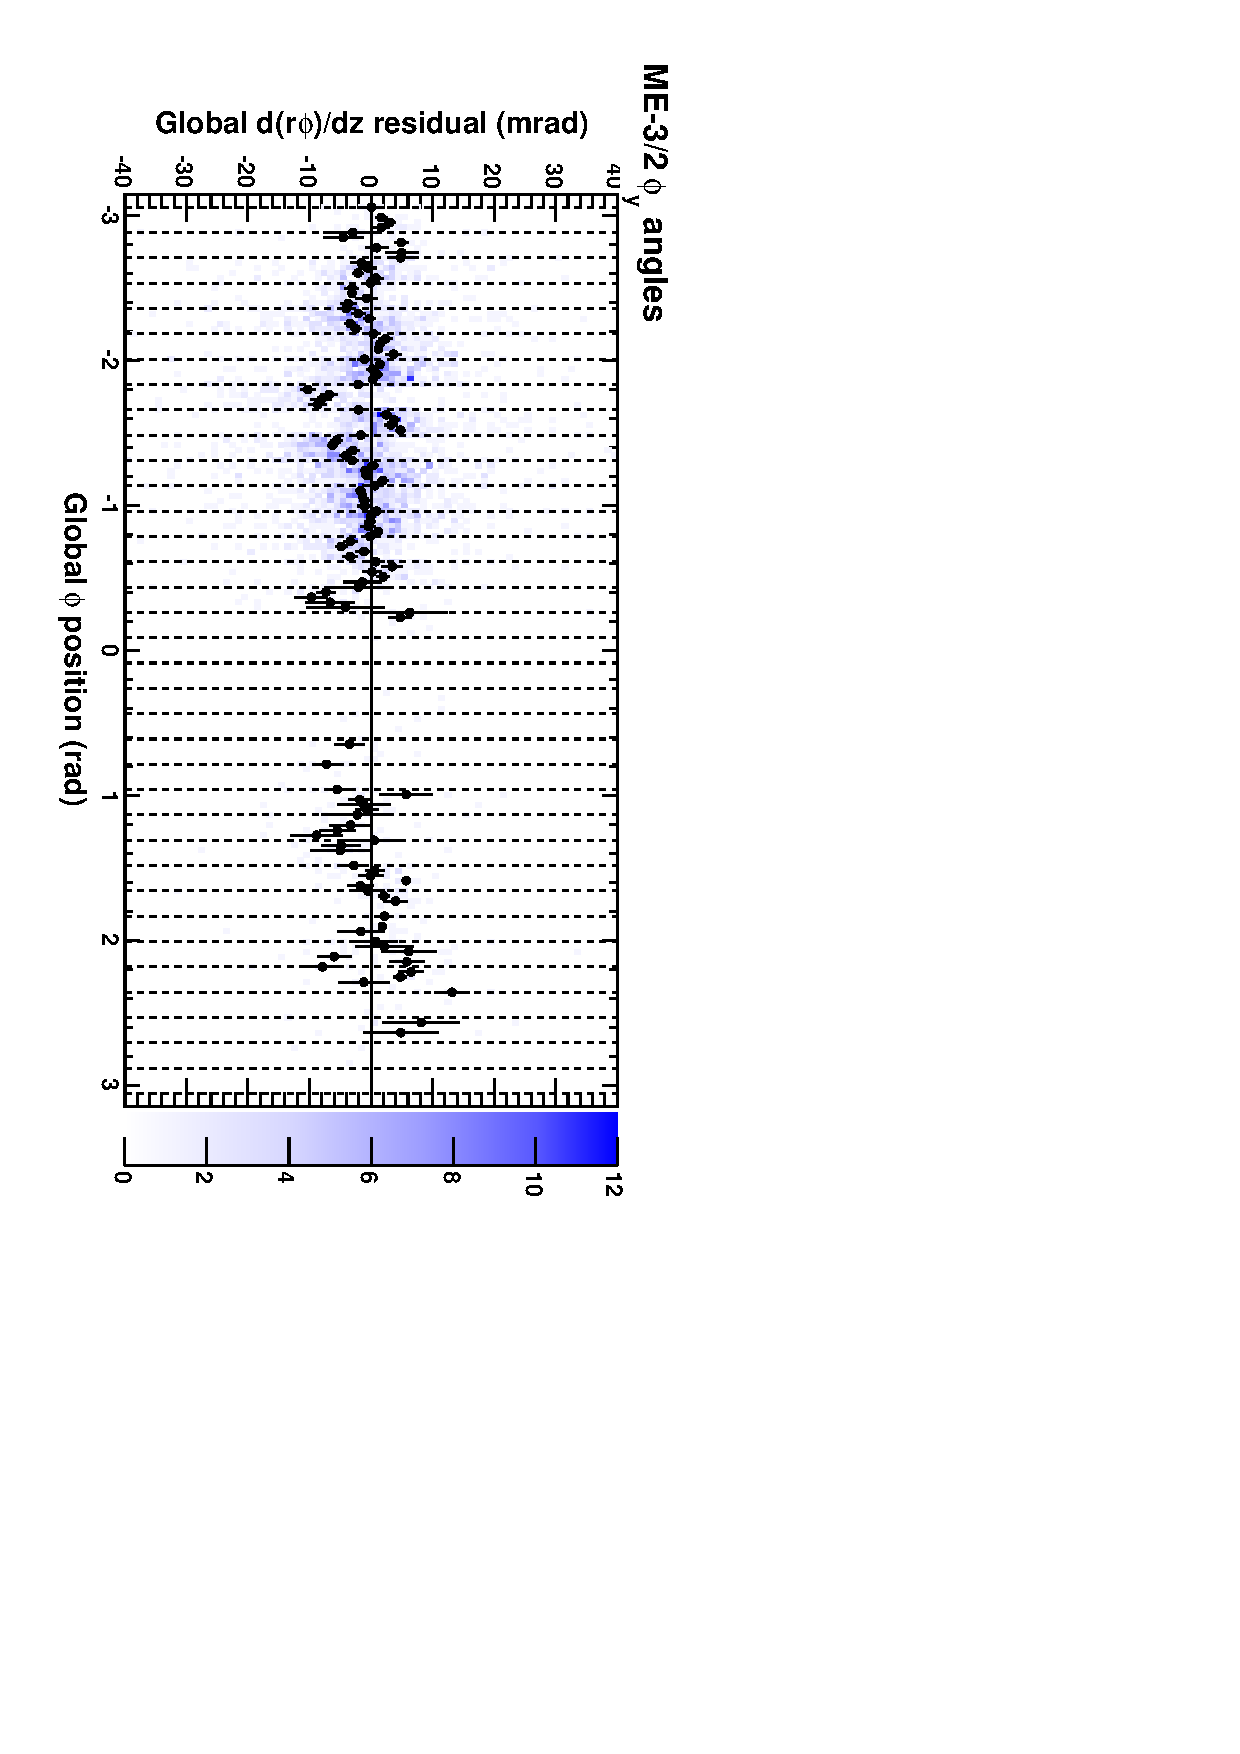
\includegraphics[height=\linewidth, angle=90]{datacsc_all_mep32phiy.pdf}}

\end{frame}

\begin{frame}
\frametitle{Comparison with beam-halo}
\begin{itemize}\setlength{\itemsep}{0.25 cm}
\item Difficult to actually compare tracker-to-disk and beam-halo directly, because very few cosmic rays connect ME$-$2/1 with the tracker
\item Nevertheless, we can try: these are $\phi_y$ with \textcolor{red}{beam-halo} overlaid

\begin{center}
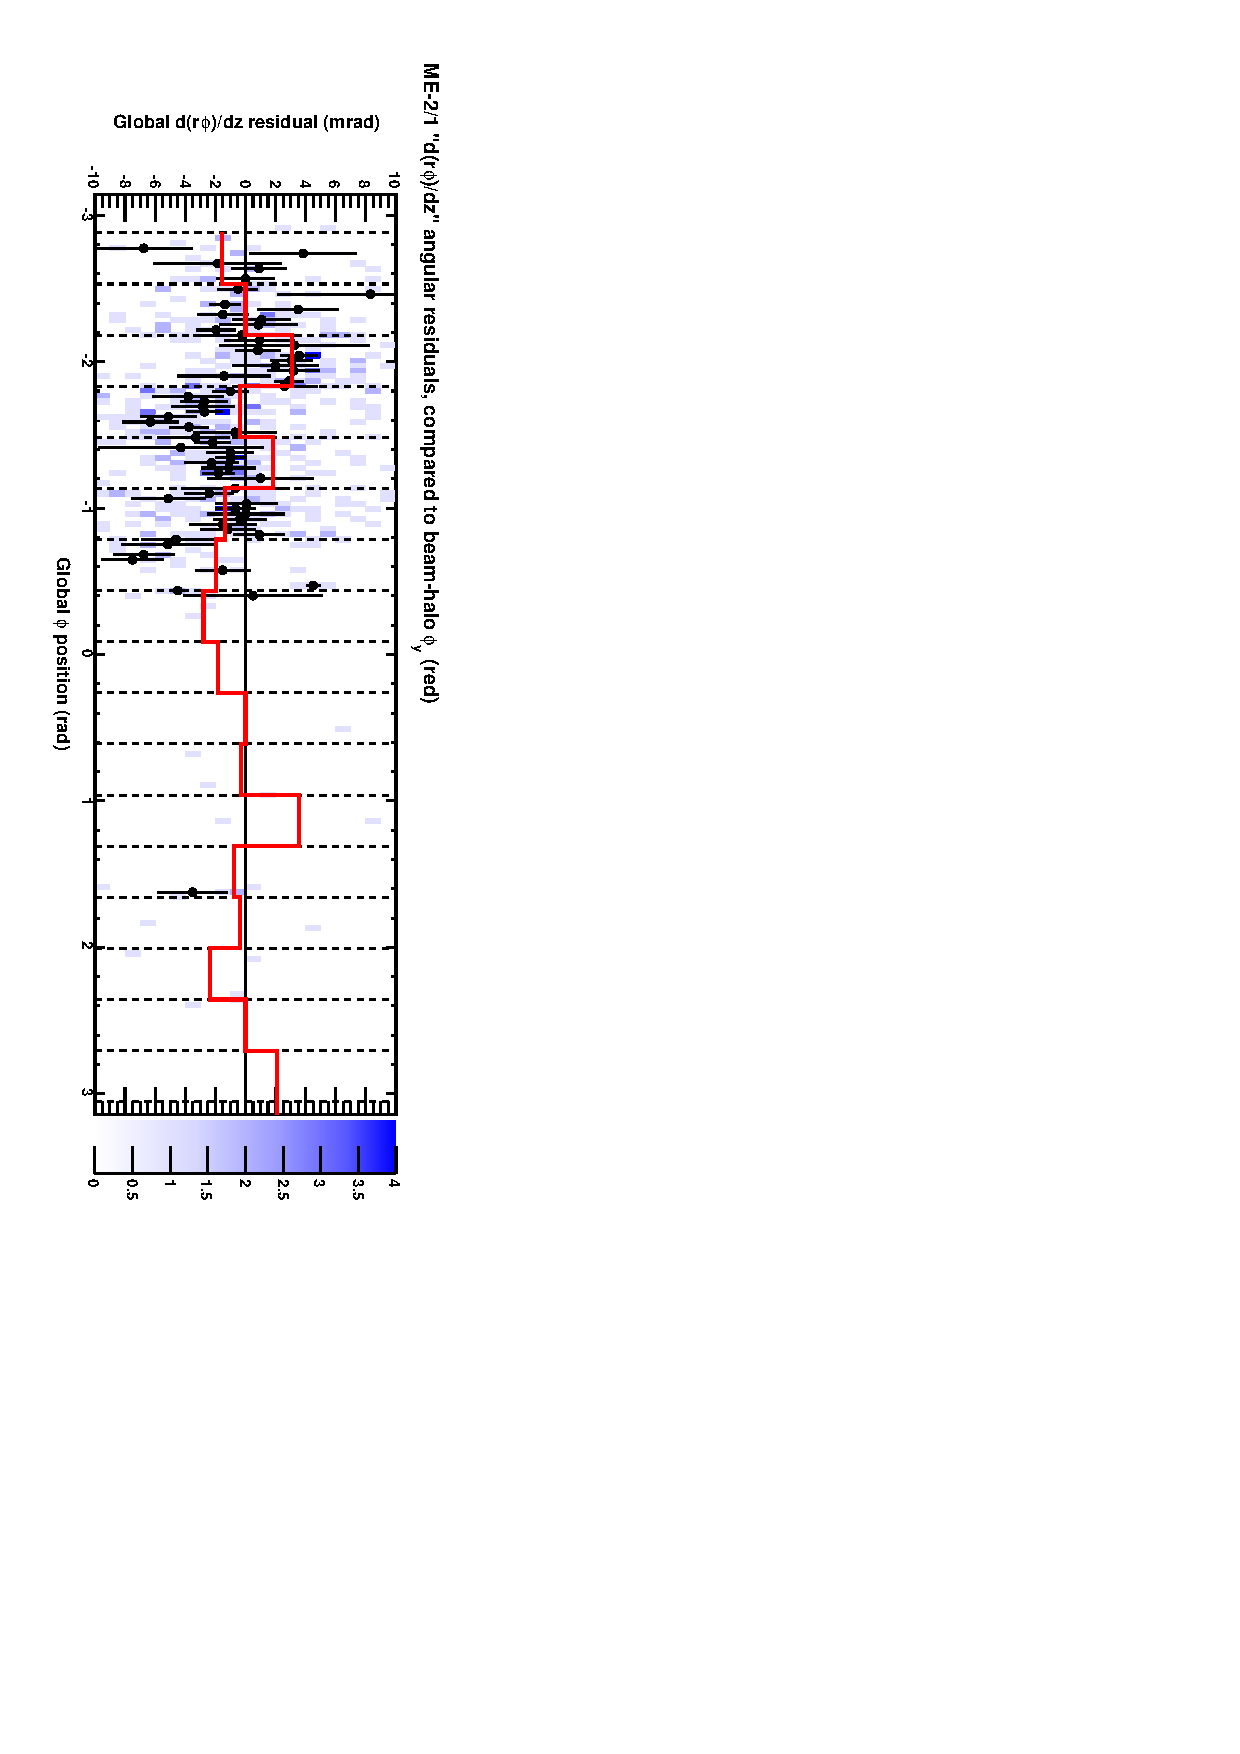
\includegraphics[height=\linewidth, angle=90]{datacsc_phiy_andbeamhalo.pdf}
\end{center}

\item To allow for tracker distortions and propagator errors, we can focus on the discontinuities at the chamber boundaries
\item The discontinuities do not agree in detail with beam-halo: can form an argument that chambers have rotated between \mbox{$\vec{B}=0$ and CRAFT\hspace{-1 cm}}
\end{itemize}
\end{frame}

\begin{frame}
\frametitle{How does it look in MC?}

\begin{itemize}\setlength{\itemsep}{0.25 cm}
\item Collisions MC (5~pb$^{-1}$): tracks uniform in $\phi$ but not more numerous
\item Much easier to fit const $+$ sine $+$ cosine, accurate results
\item Roughly the same residuals widths

\vspace{0.5 cm}
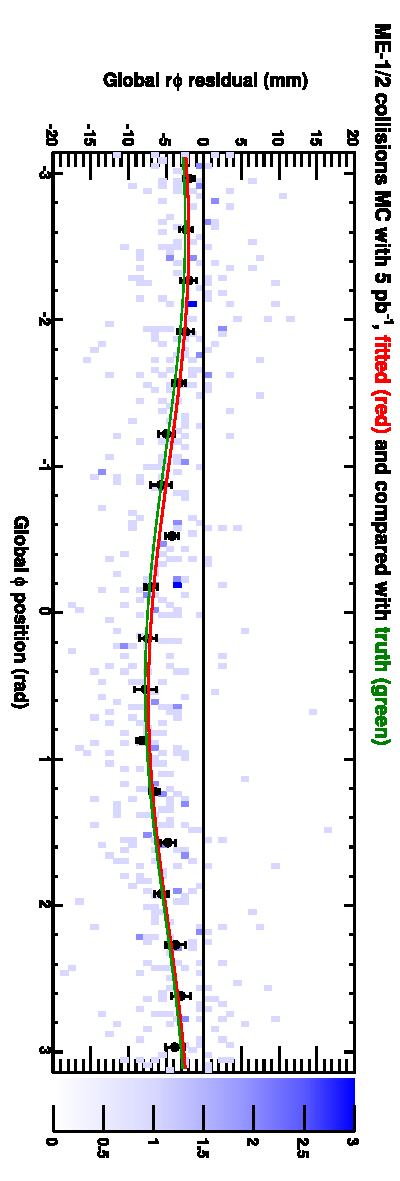
\includegraphics[height=\linewidth, angle=90]{mccsc_example_5pb.pdf}

\item Cosmic-ray MC (full sample): zero tracks {\scriptsize (probably a generator-level cut)}
\end{itemize}
\end{frame}

\begin{frame}
\frametitle{MC disk-fitting study}
\begin{itemize}
\item With $\phi$-symmetric collisions, how much data do we need to align the disks?
\item Includes residual misalignments after CSC Overlaps alignment (assuming same resolution as 2008)
\item Independent samples scale with $\sqrt{N}$
\end{itemize}

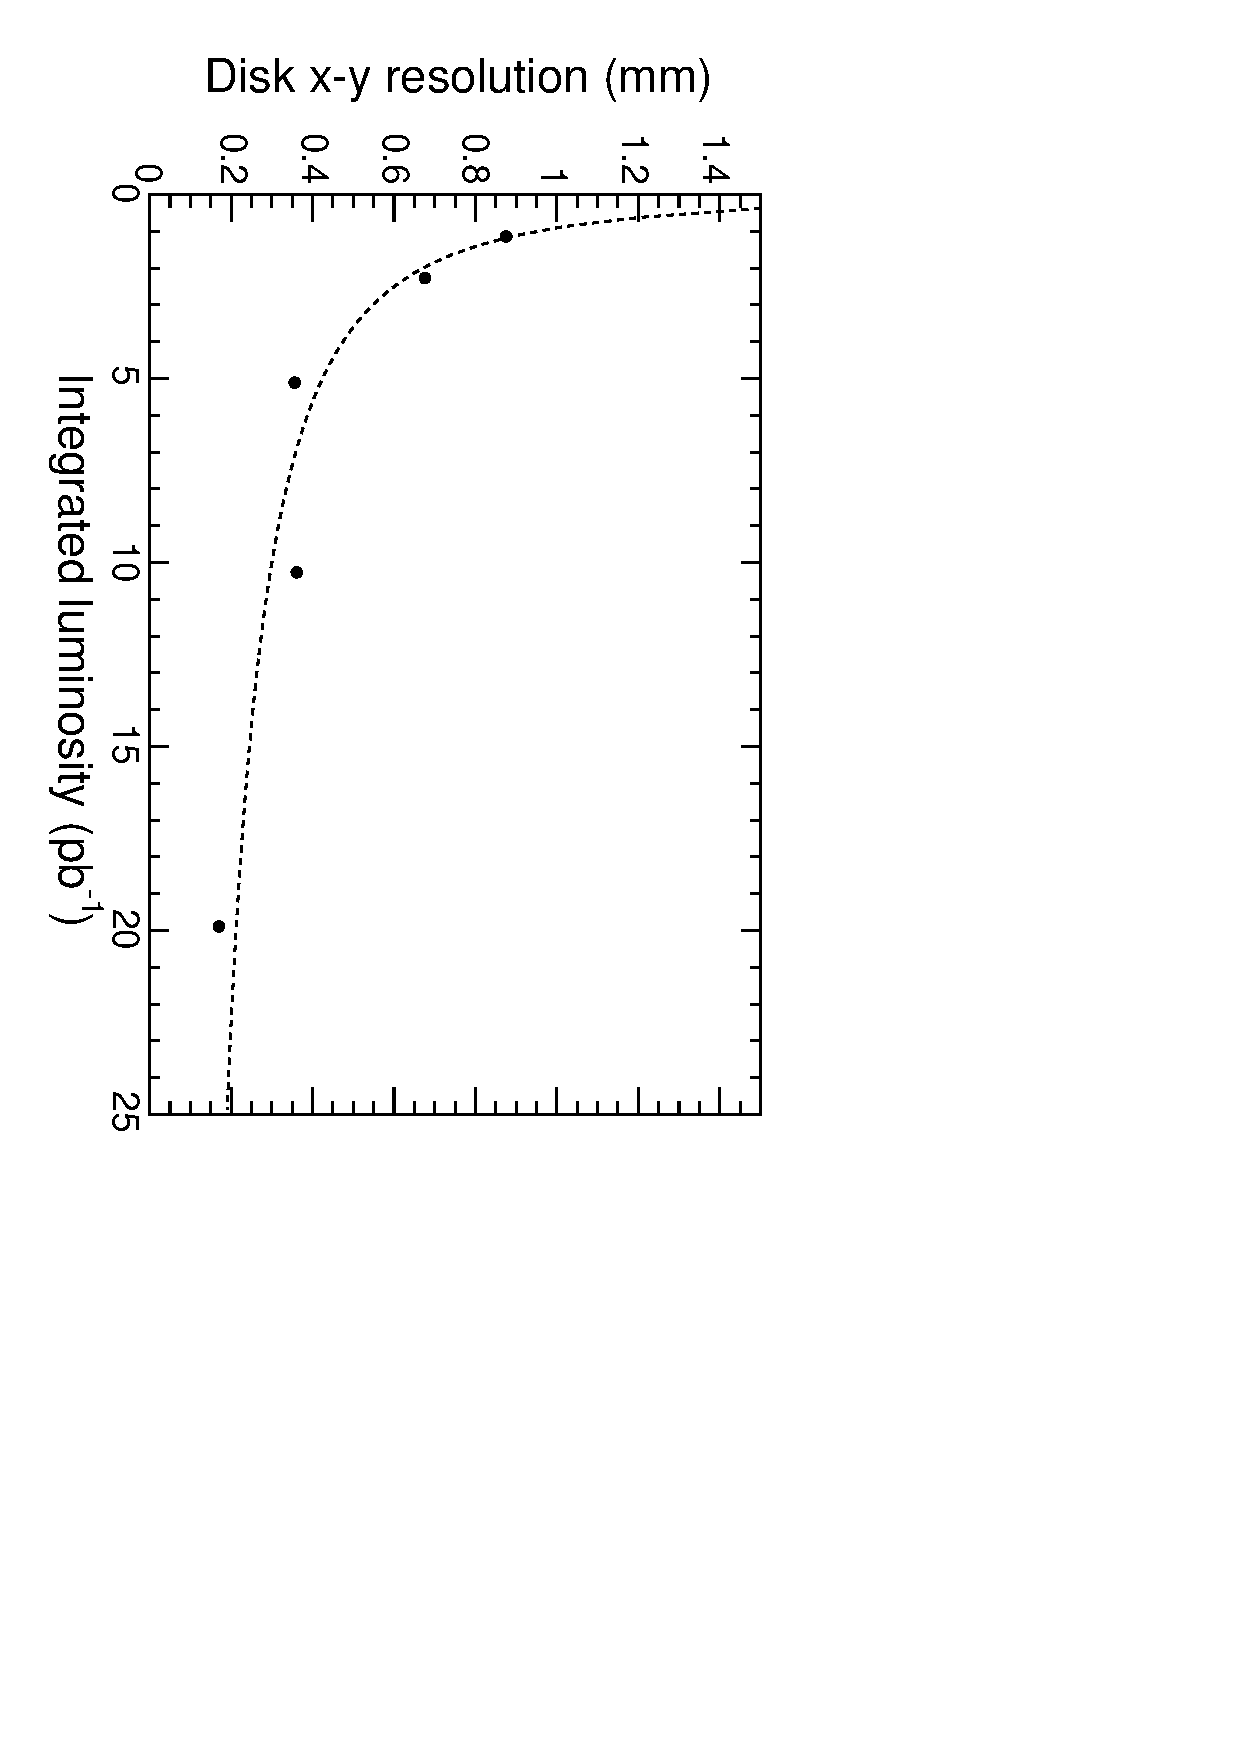
\includegraphics[height=0.5\linewidth, angle=90]{mccsc_diskstats_xy.pdf}
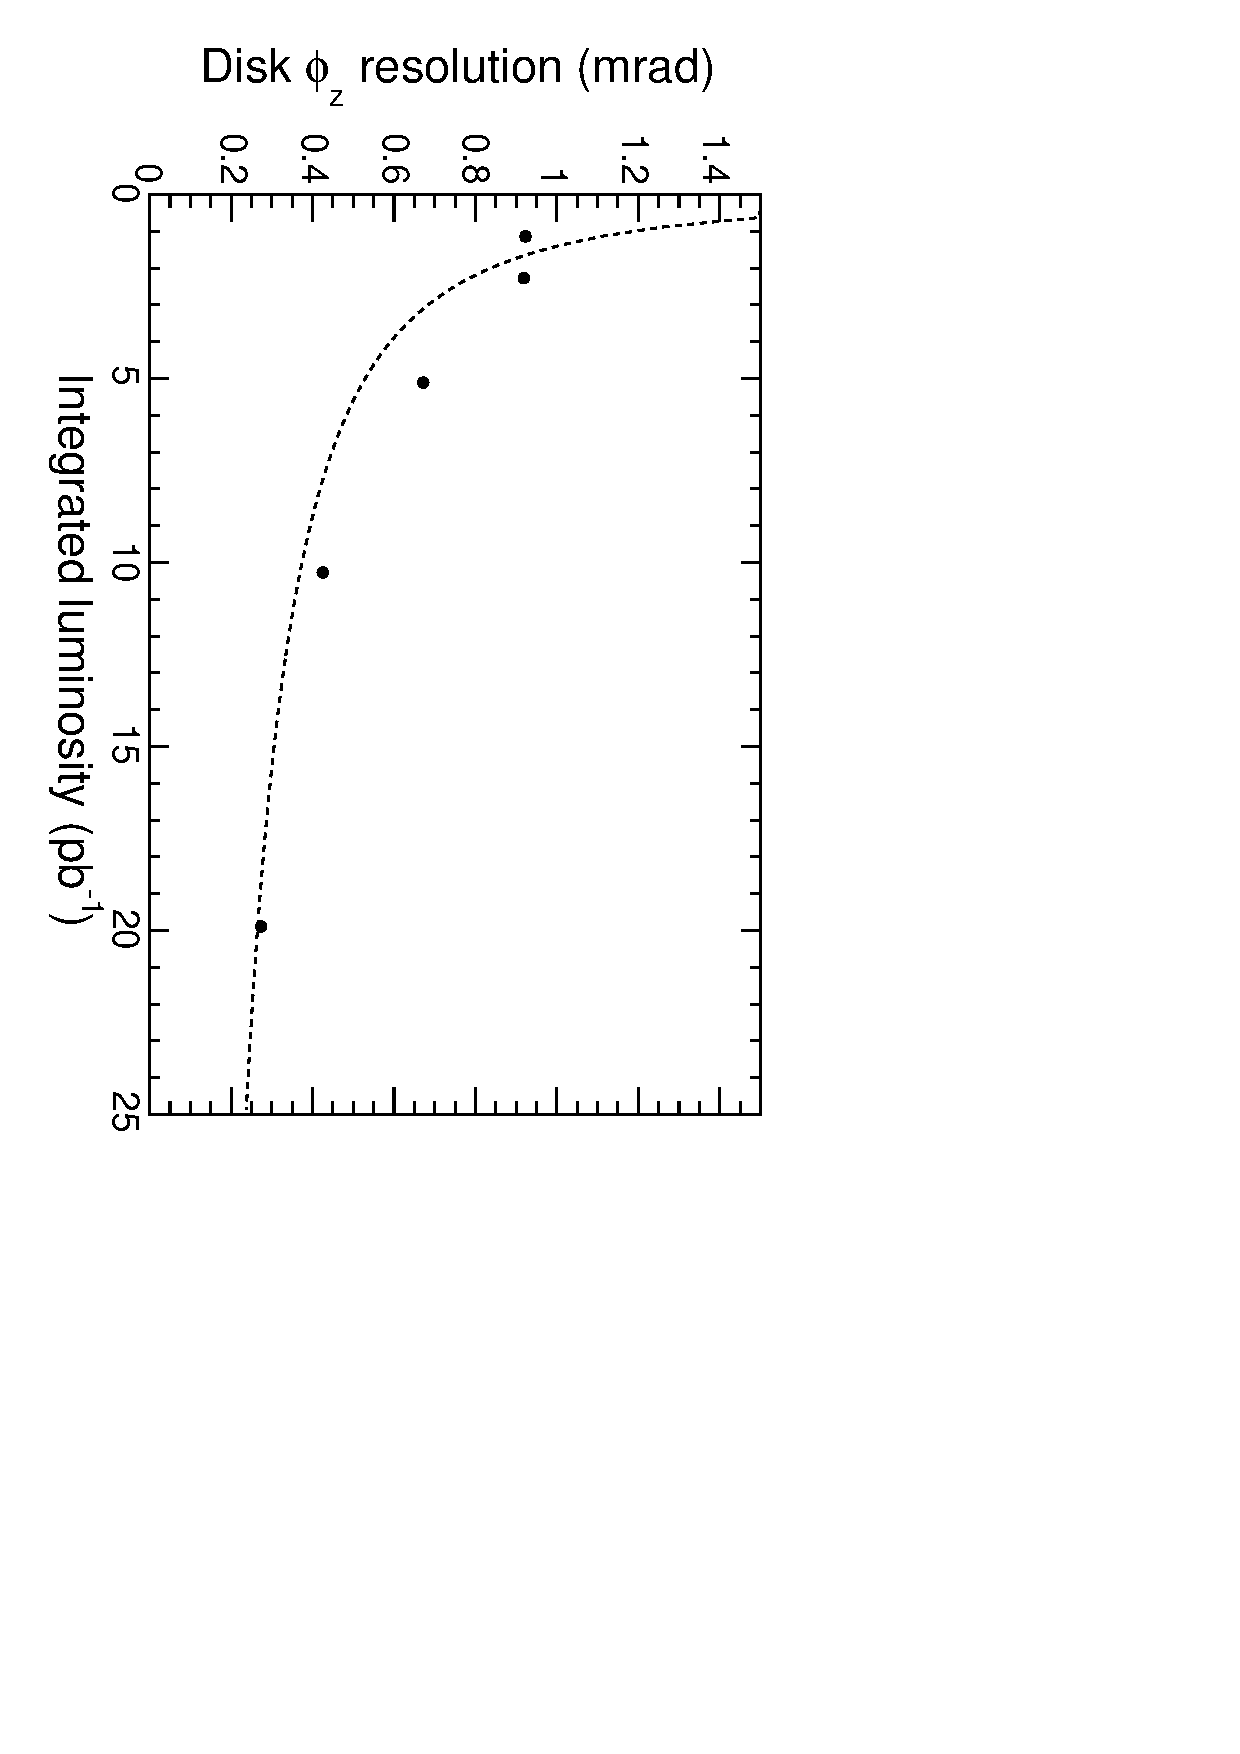
\includegraphics[height=0.5\linewidth, angle=90]{mccsc_diskstats_phiz.pdf}

\begin{itemize}
\item This is a walk-through of what we'll need to do after CSC Overlaps
\end{itemize}
\end{frame}

\section*{Conclusions}

\begin{frame}
\frametitle{Timeline for beam}
\scriptsize
\begin{itemize}
\item Now and CRAFT-2009
\begin{itemize}
\item \scriptsize validate cosmic ray tracker-to-disk procedures with CRAFT-2008 \mbox{and -2009\hspace{-1 cm}}
\item \scriptsize automate all procedures and monitoring for CRAFT-2009, then simply run them
\end{itemize}

\item Month of beam-halo only
\begin{itemize}
\item \scriptsize re-run beam-halo procedure on new samples
\item \scriptsize kludge incomplete rings if necessary
\item \scriptsize any corrections needed for $\vec{B} \ne 0$?
\item \scriptsize one-time layer alignment with full dataset \\ {\scriptsize (low-statistics 2008 pilot study on right)}
\end{itemize}

\vspace{-2.90 cm}
\hfill 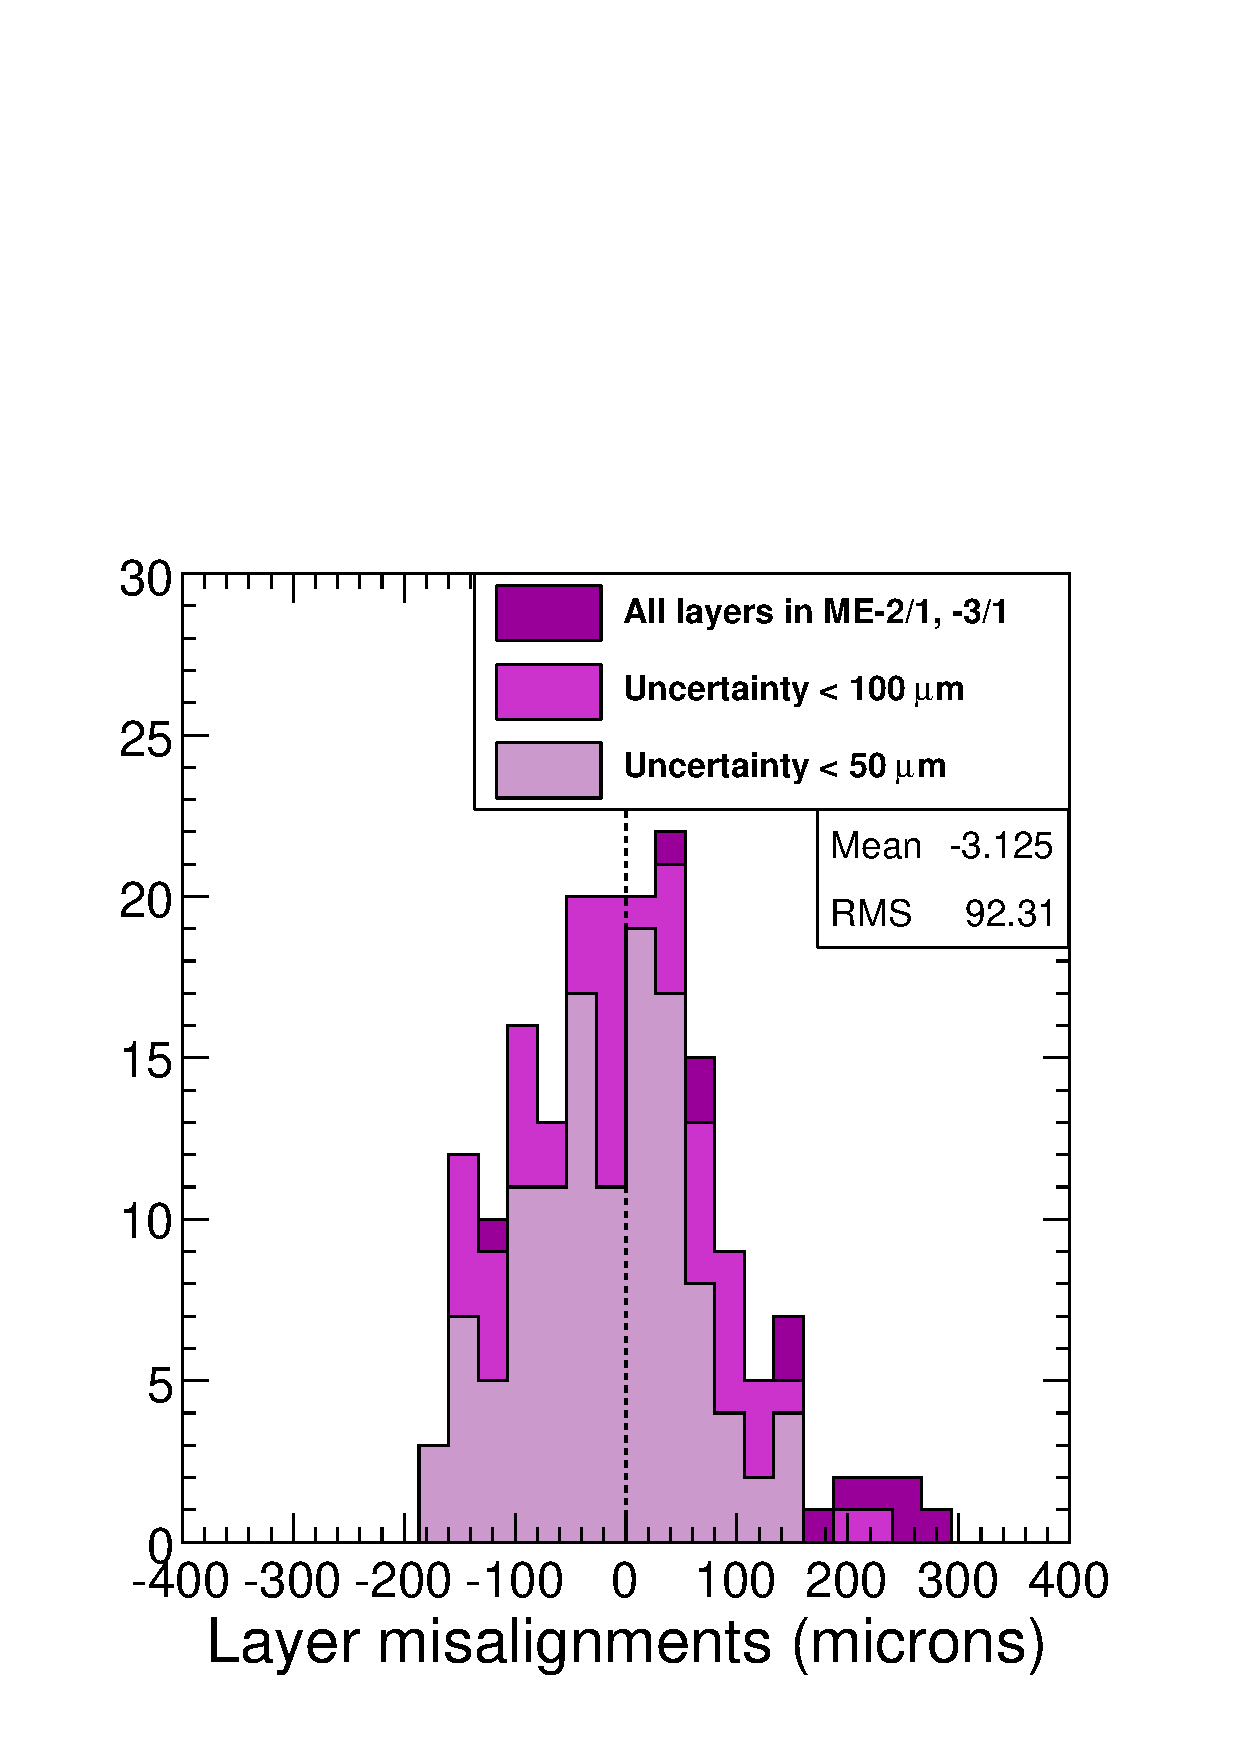
\includegraphics[width=0.3\linewidth]{layer_hist.pdf}

\vspace{-1.20 cm}
\mbox{ }

\item First collisions: 5~pb$^{-1}$
\begin{itemize}
\item \scriptsize run Overlaps procedure on collisions data, compare with beam-halo result
\item \scriptsize use tracker-to-disk method to connect internally-aligned rings to tracker
\end{itemize}

\item Later collisions: 50~pb$^{-1}$
\begin{itemize}
\item \scriptsize run Baseline procedure with same tracks: do they agree?  If not, do track-by-track comparisons to diagnose the problem
\item \scriptsize do collisions alignments agree with cosmic rays in the barrel?
\end{itemize}
\end{itemize}
\end{frame}

\begin{frame}
\frametitle{Conclusions}

\begin{itemize}\setlength{\itemsep}{0.25 cm}
\item Cosmics-during-collisions trigger is important, and it's getting built
\item No clear convergence on endcap alignment yet, but hints of regional agreement
\item globalMuons ME2/2 and ME3/2 agree with each other
\item $\phi_y$ misalignments clearly seen, on the scale of what we saw
  in beam-halo, but not a good correlation: movement when $\vec{B} \to
  3.8$~T?
\item Collisions MC yields a much easier-to-fit disk due to $\phi$ symmetry of hits
\end{itemize}

\label{numpages}
\end{frame}

\end{document}
